\documentclass[xcolor={dvipsnames},aspectratio=169,10pt]{beamer}
\usetheme{mx}
\usepackage{graphicx}
\graphicspath{{../figures}}
%\input{preamble.tex}

\title{
%Teaching AI and Robotics to Children in a Mexican town
Ense\~nando Inteligencia Artificial y Rob\'otica \\ 
en un pueblo Mexicano \\
}
\subtitle{
Taller de diversidad, equidad e inclusi\'on (DEI-HRI2023) 
}

\author{
Antonio Badillo-P\'erez,
Donato Badillo-P\'erez, 
Alex Barco, \\ 
Rocio Montenegro, and
{\bf Miguel Xochicale}
}

\date{
%12th March 2023
}

\institute{
	\faEnvelope \space  air4children@gmail.com \\
	\faGithubAlt \space @air4children \faTwitter \space @air4children  
		}
\githubrepository{https://github.com/air4children/dei-hri2023}


\begin{document}

\maketitle

\begin{frame}{Contenido}
    \tableofcontents
\end{frame}

%%%%%%%%%%%%%%%%%%%%%%%%%%%%%%%%%%%%%%%%%%%%
\section{Contexto}


\begin{frame}
      \frametitle{Contenido}
      \tableofcontents[currentsection]
\end{frame}

%%%%%%%%%%%%%%%%%%%%%%%%%%%%%%%%%%%%%%%%%%%%%
%\subsection{Education programs, publications and private investment in AI and Robotics}
\subsection{Educaci\'on, investigaci\'on e inversi\'on privada en IA y Rob\'otica}

%%%%%%%%%%%%%%%%%%%%%%%%%%%%%%%%%%%%%%%%%%%%%%%%%%%%%%%%
{
%\paper{Savage N. 2021 in Nature, DOI: doi.org/10.1038/d41586-020-03409-8}
\paper{Zhang D. et al 2021 in AI 2021 Index Report, Fig 4.3.3 \url{https://aiindex.stanford.edu/report/}}

\begin{frame}{
Programas en IA por \'area geogr\'afica y nivel educativo, 2019-2020
}

\begin{figure}
 \centering
 \includegraphics[width=1.0\textwidth]{./progress-of-air-a0/outputs/drawing-v00.png}
 %\caption{}
\end{figure}

\end{frame}
}

%%%%%%%%%%%%%%%%%%%%%%%%%%%%%%%%%%%%%%%%%%%%%%%%%%%%%%%%
{
%\paper{Savage N. 2021 in Nature, DOI: doi.org/10.1038/d41586-020-03409-8}
%\paper{Zhang D. et al 2021 in AI 2021 Index Report, Fig 1.1.19 \url{https://aiindex.stanford.edu/report/}}
\paper{AI Index Report 2022, Fig 4.2.4 \url{https://aiindex.stanford.edu/report/}}

\begin{frame}{
%Private investment in AI by Geographic area
Inversion privada en IA por \'area geogr\'afica, 2021
}

\begin{figure}
 \centering
 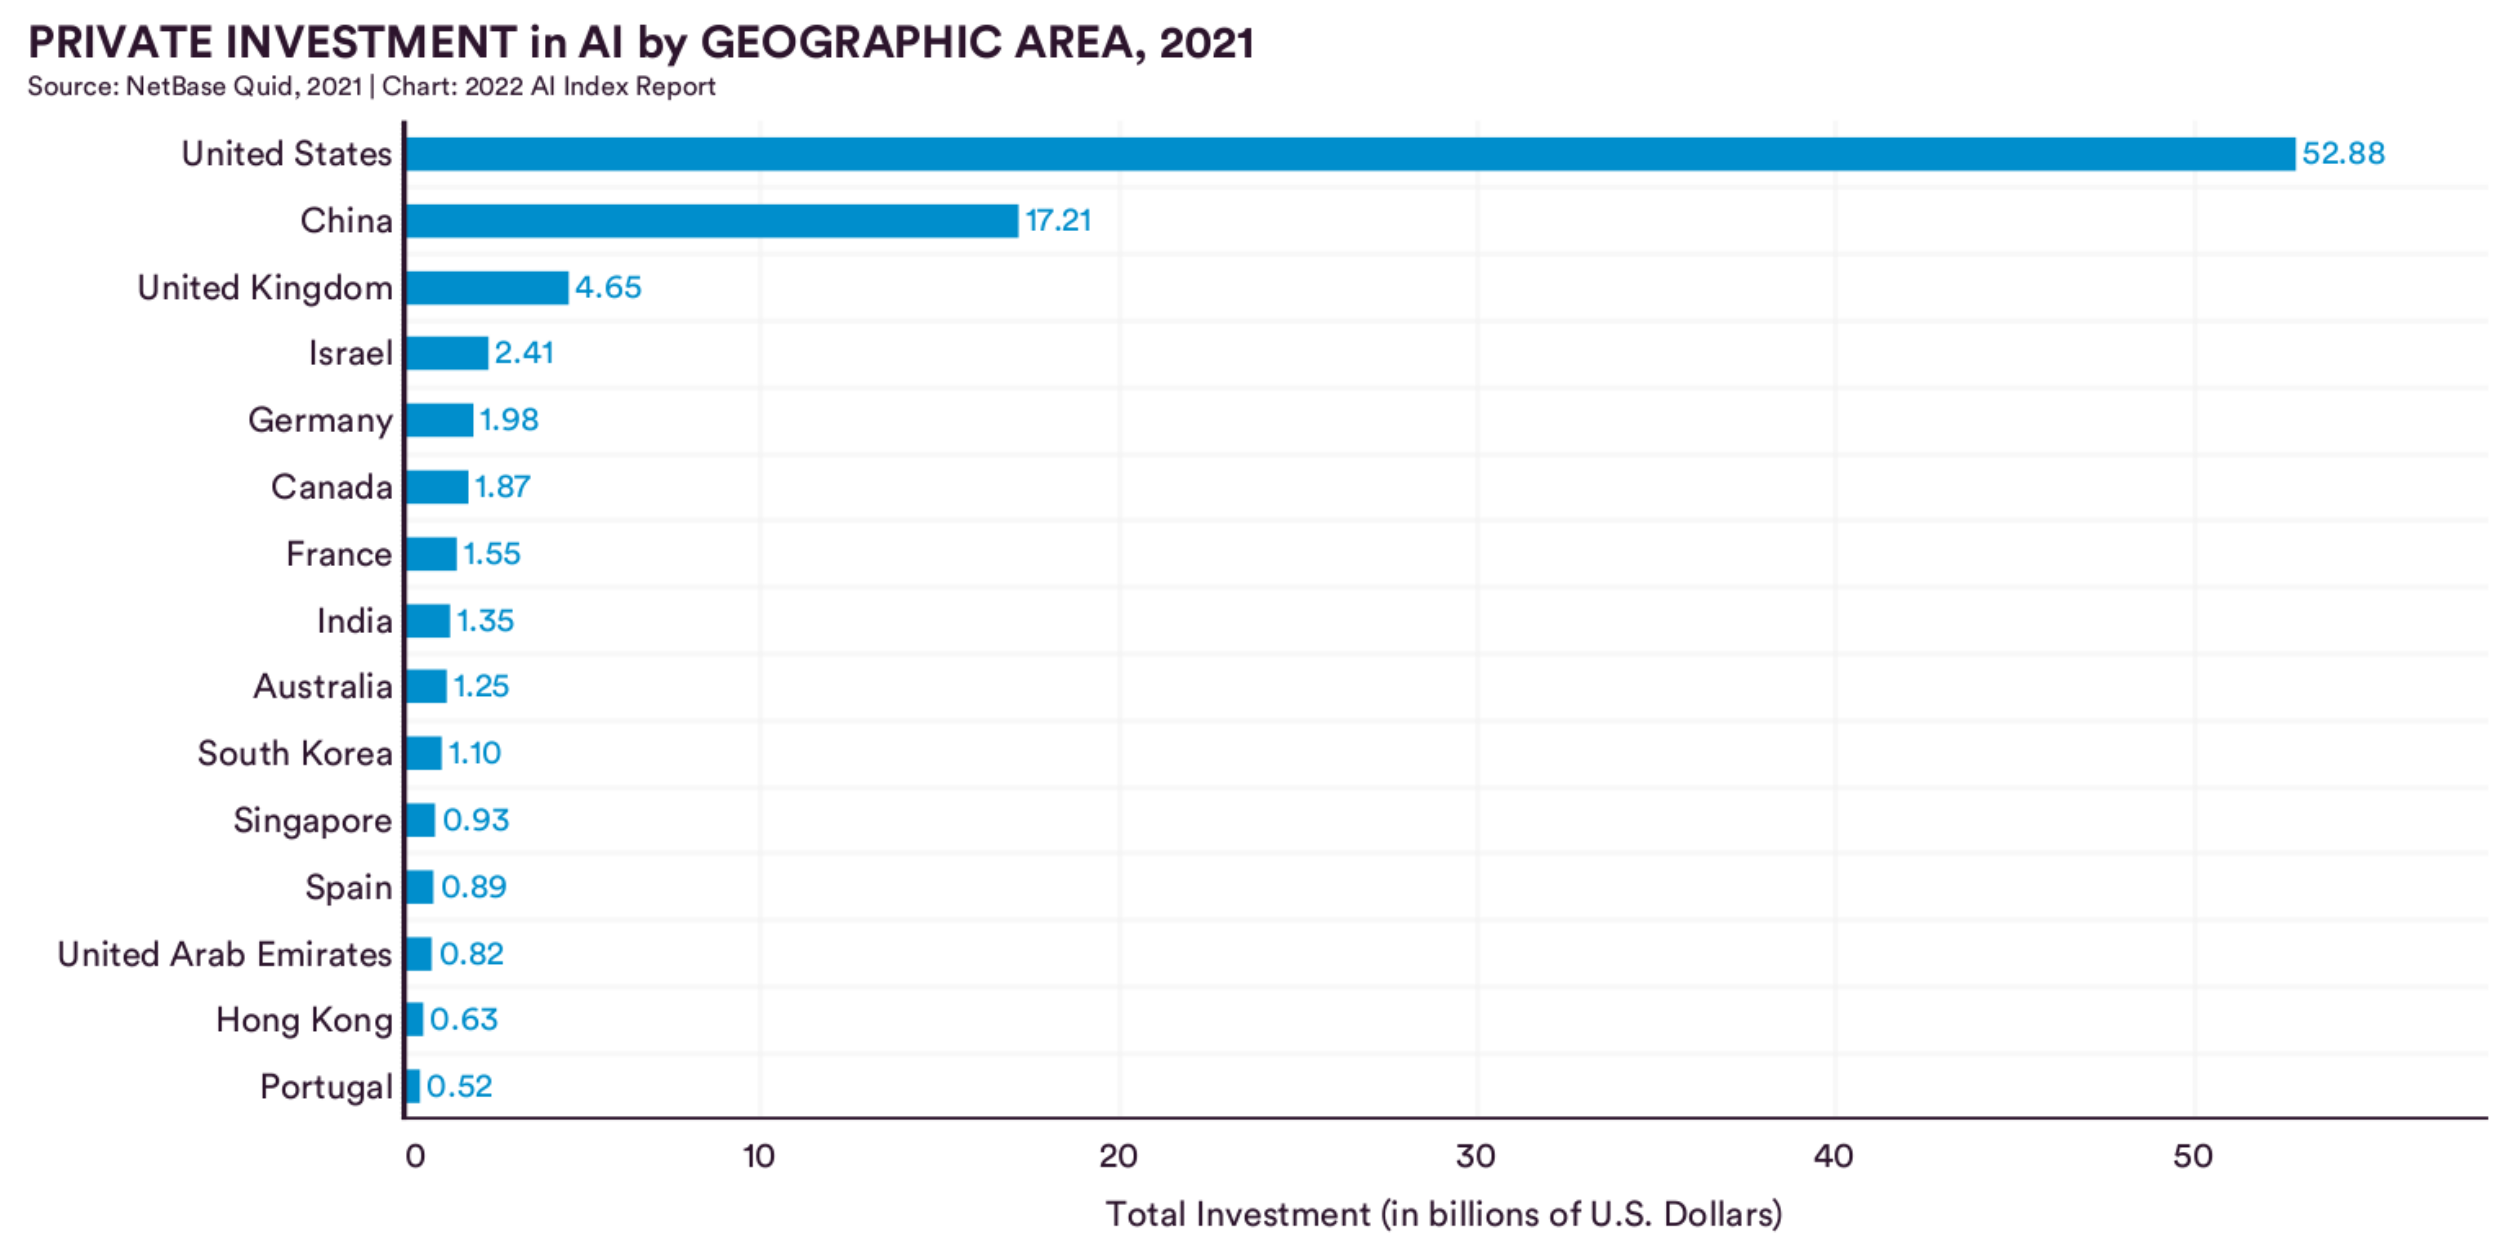
\includegraphics[width=1.0\textwidth]{./progress-of-air-c/outputs/drawing-v01.png}
 %\caption{}
\end{figure}

\end{frame}
}



%%%%%%%%%%%%%%%%%%%%%%%%%%%%%%%%%%%%%%%%%%%%%%%%%%%%%%%%%
%{
%%\paper{Savage N. 2021 in Nature, DOI: doi.org/10.1038/d41586-020-03409-8}
%\paper{AI Index Report 2022, Fig 4.4.4 \url{https://aiindex.stanford.edu/report/}}
%
%\begin{frame}{New CS PhDs with AI/ML and Robotics/Vision Specialties}
%
%\begin{figure}
% \centering
% \includegraphics[width=1.0\textwidth]{./figures/progress-of-air-a1/outputs/drawing-v00.png}
% %\caption{}
%\end{figure}
%
%\end{frame}
%}
%
%

%%%%%%%%%%%%%%%%%%%%%%%%%%%%%%%%%%%%%%%%%%%%%%%%%%%%%%%%%
%{
%%\paper{Savage N. 2021 in Nature, DOI: doi.org/10.1038/d41586-020-03409-8}
%%\paper{Zhang D. et al 2021 in AI 2021 Index Report, Fig 1.1.19 \url{https://aiindex.stanford.edu/report/}}
%\paper{AI Index Report 2022, Fig 1.1.3 \url{https://aiindex.stanford.edu/report/}}
%
%\begin{frame}{
%AI-related publications by field of study
%}
%
%\begin{figure}
% \centering
% 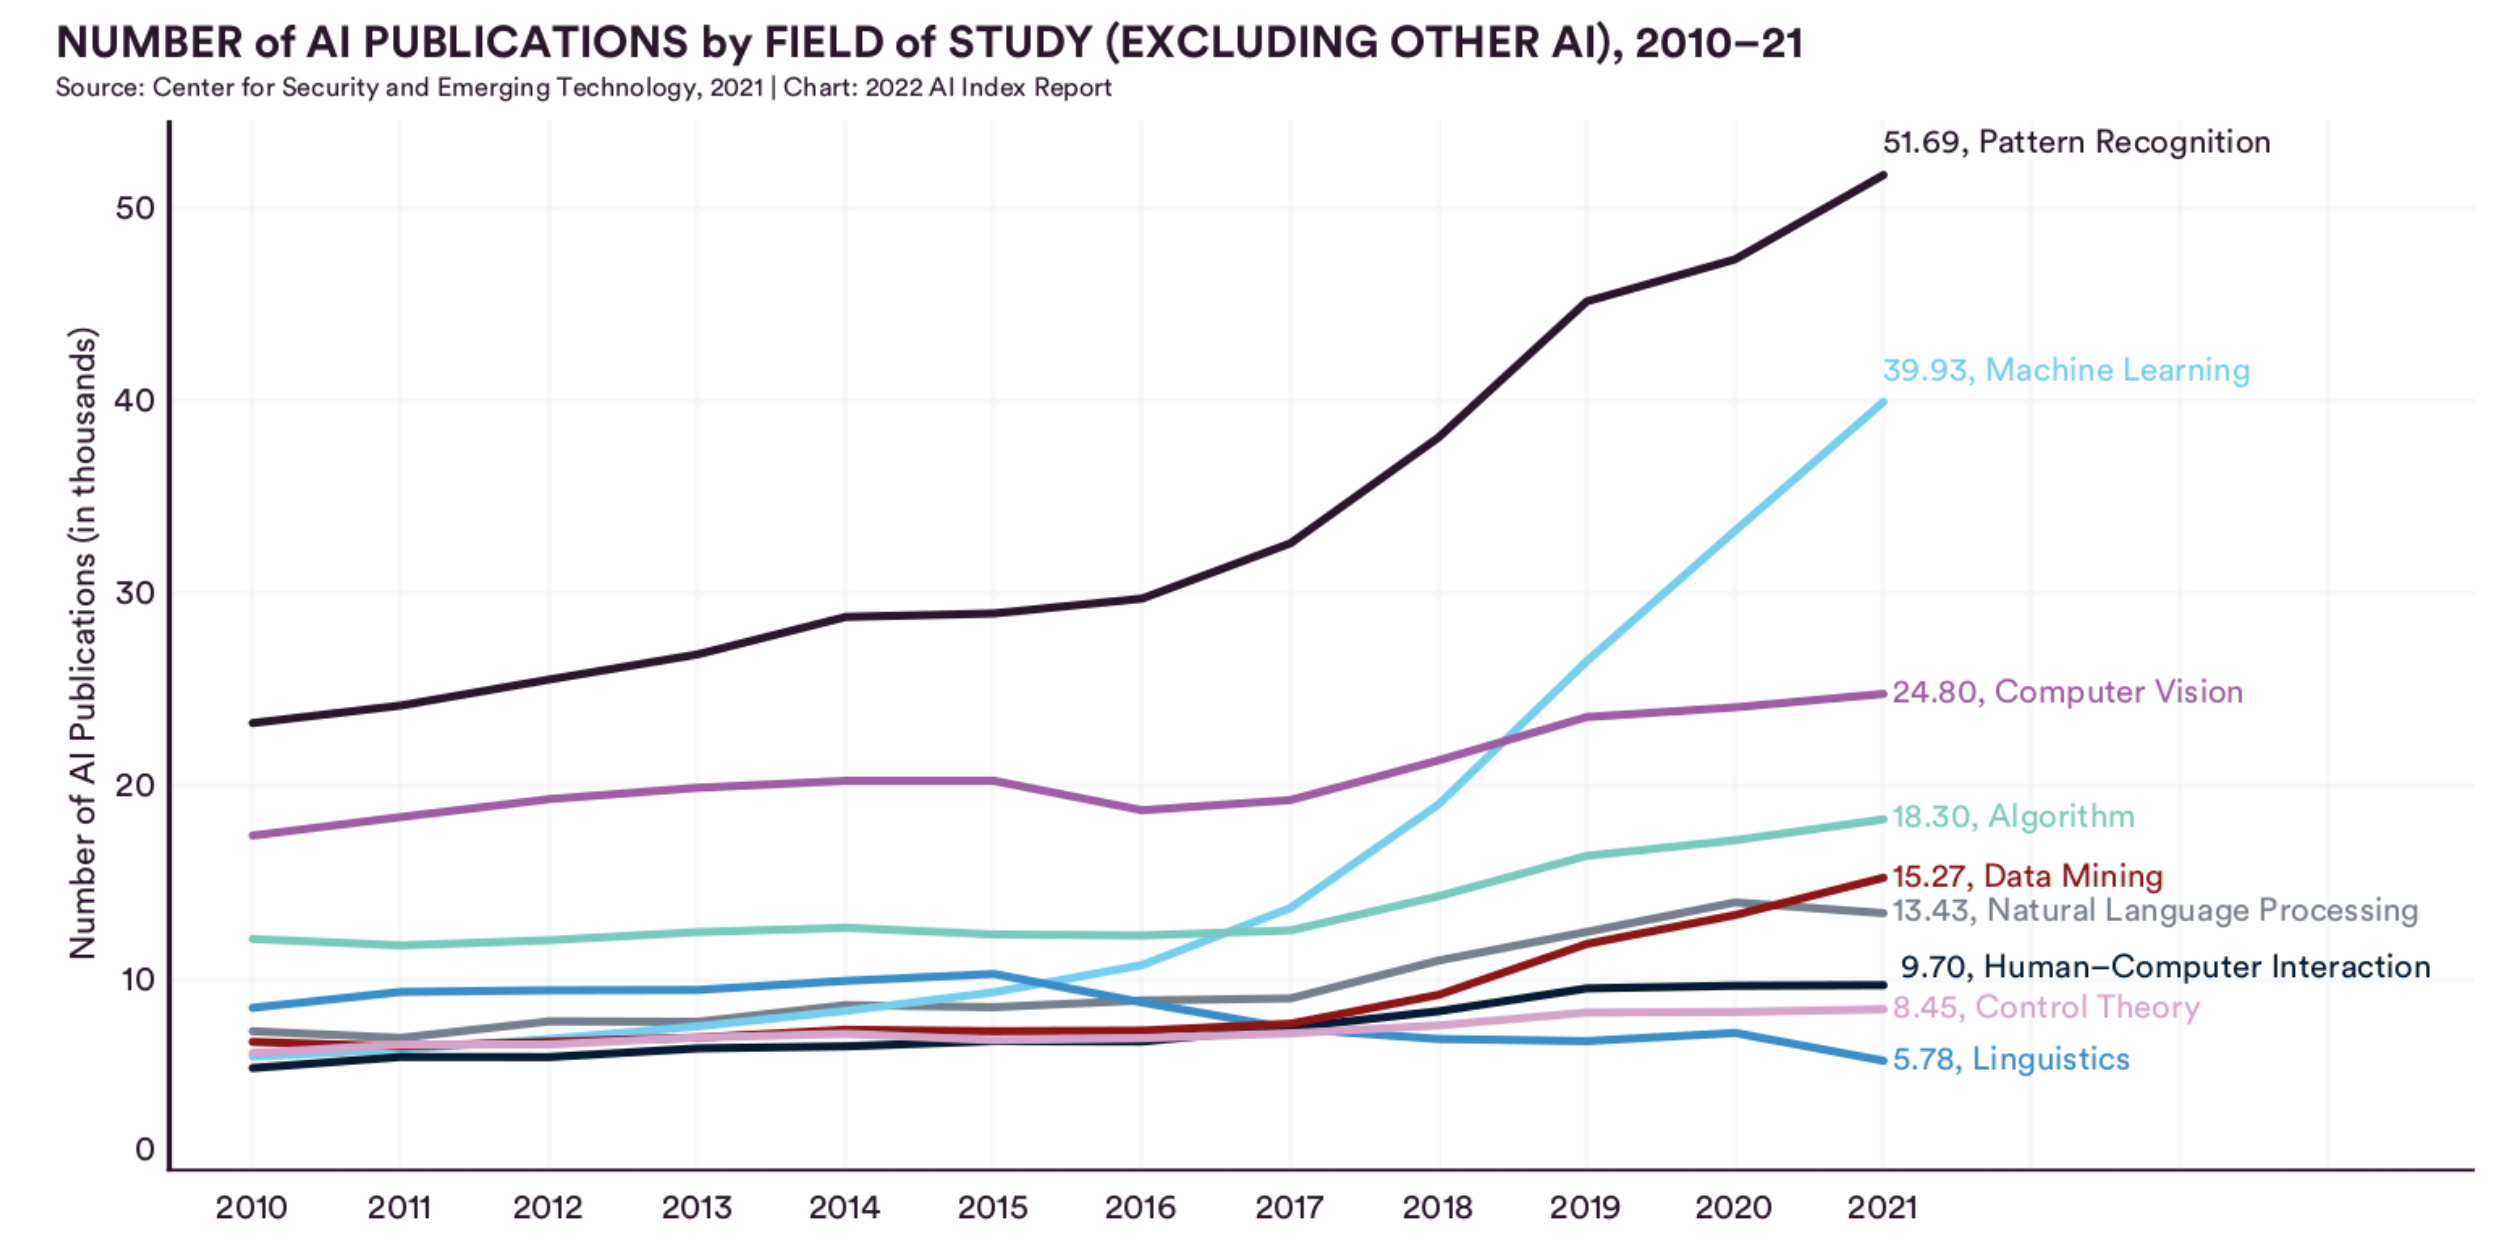
\includegraphics[width=1.0\textwidth]{./progress-of-air-b/outputs/drawing-v01.png}
% %\caption{}
%\end{figure}
%
%\end{frame}
%}
%

%%%%%%%%%%%%%%%%%%%%%%%%%%%%%%%%%%%%%%%%%%%%%%%%%%%%%%%%
{
%\paper{Savage N. 2021 in Nature, DOI: doi.org/10.1038/d41586-020-03409-8}
%\paper{Zhang D. et al 2021 in AI 2021 Index Report, Fig 1.1.19 \url{https://aiindex.stanford.edu/report/}}
\paper{AI Index Report 2022, Fig 3.3.7 \url{https://aiindex.stanford.edu/report/}}

\begin{frame}{
%Accepted papers on FAIRNESS and BIAS in AI at Neurips, 2015–21
Art\'iculos en Neurips en JUSTICIA y SESGOS en IA, 2014-21  
}

\begin{figure}
 \centering
 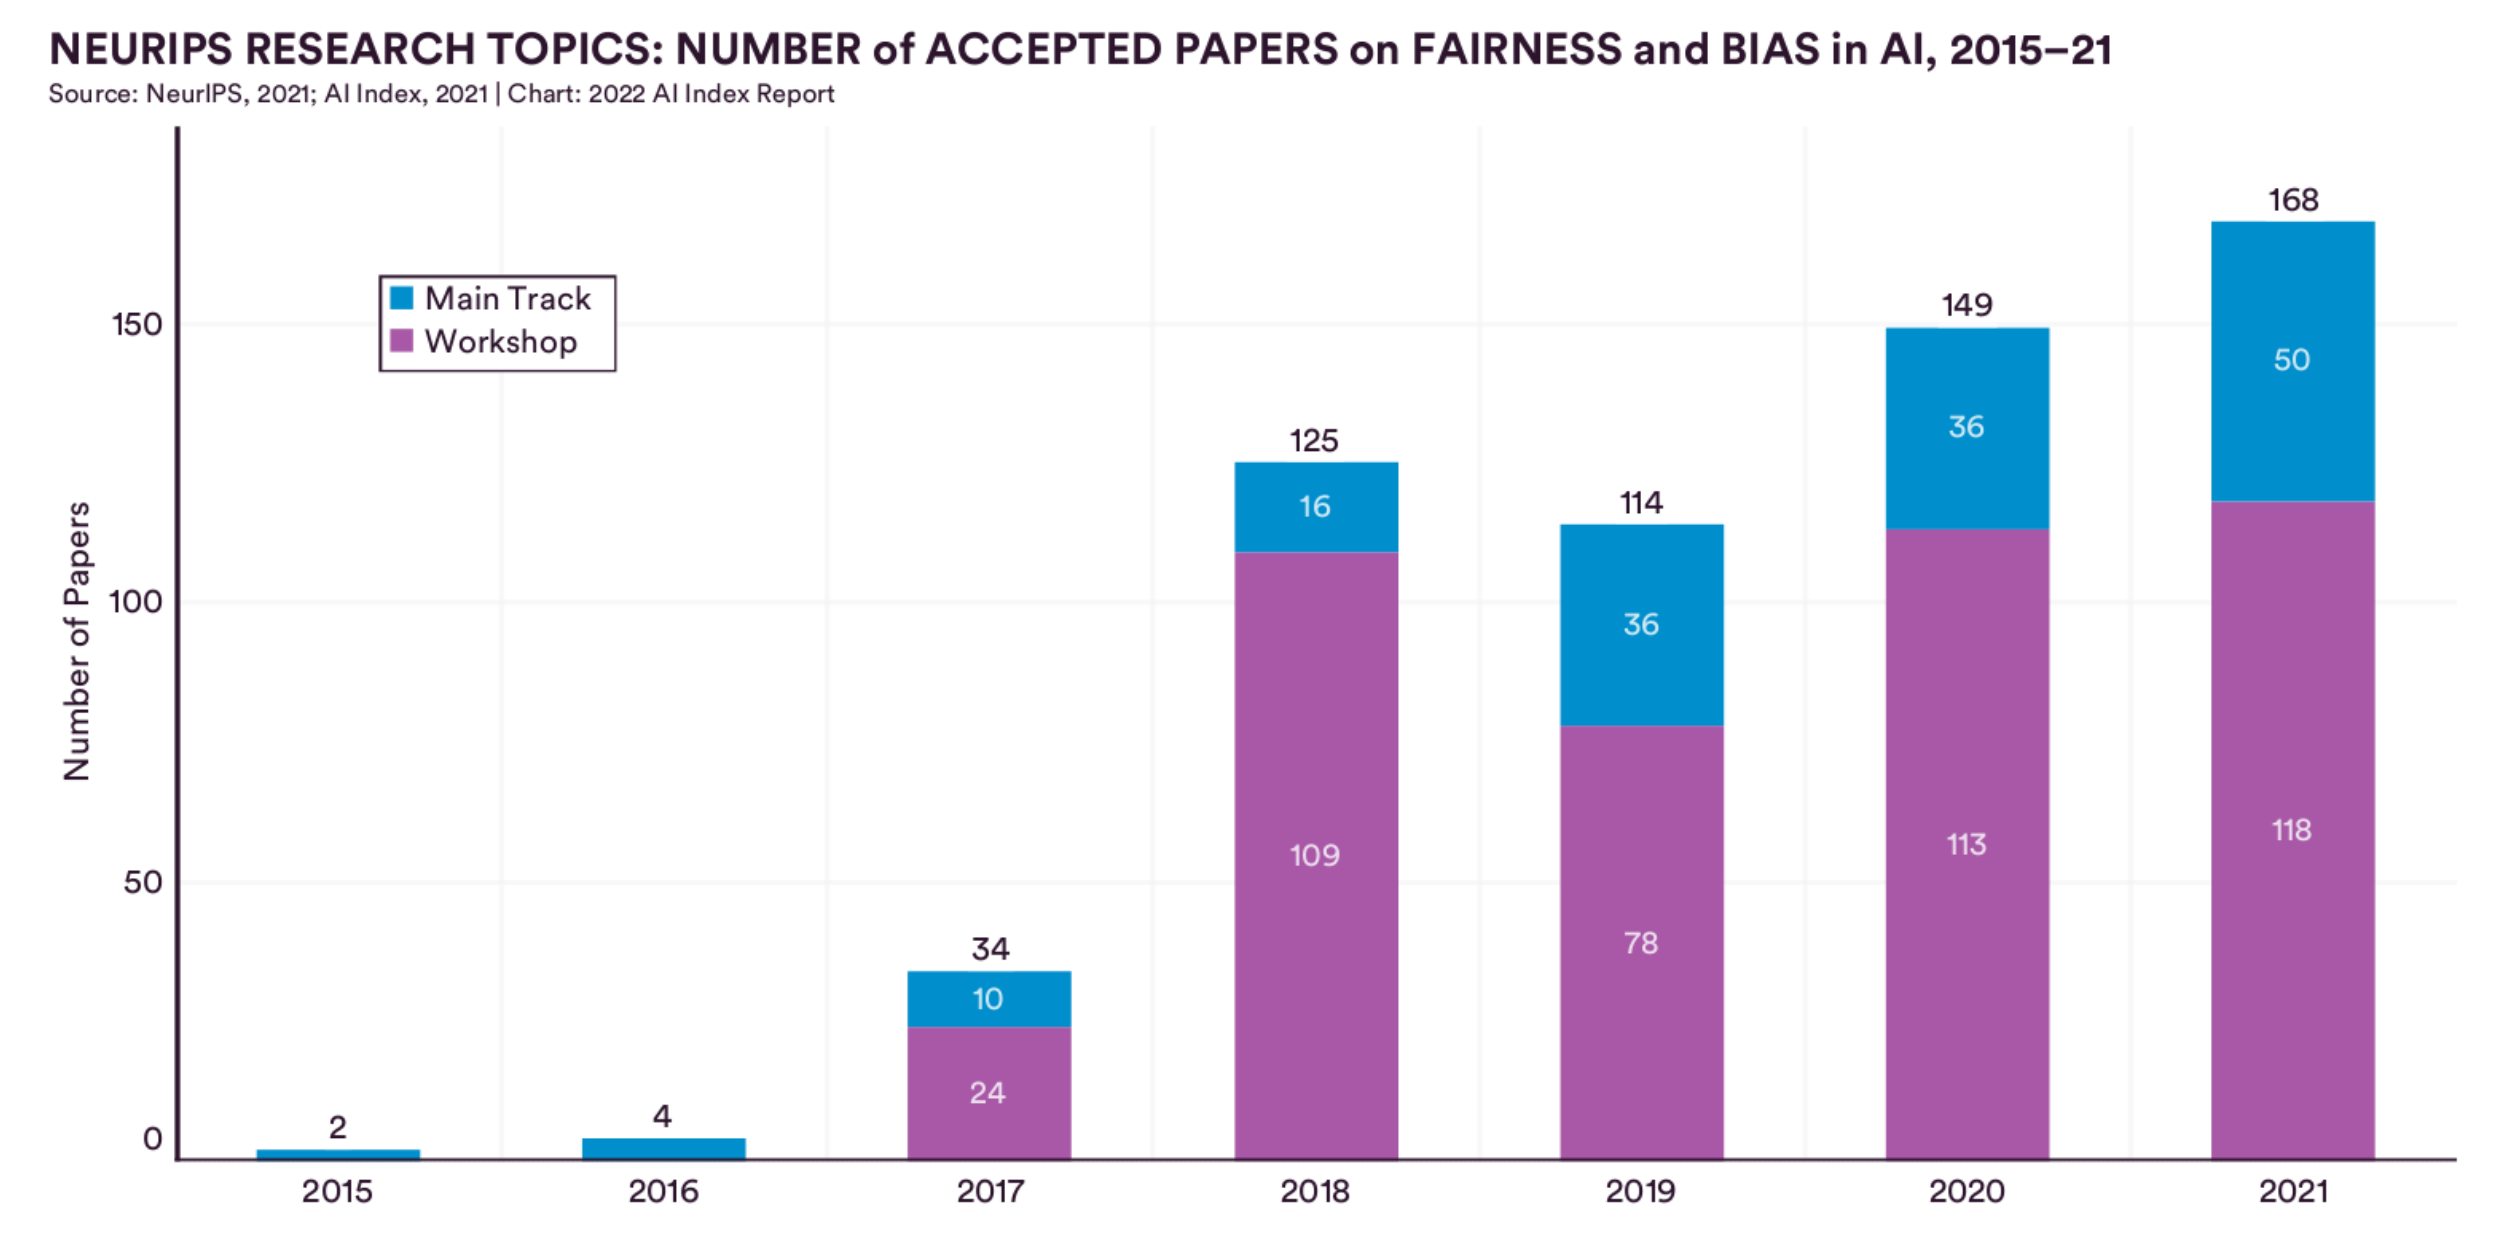
\includegraphics[width=1.0\textwidth]{./progress-of-air-d/outputs/drawing-v00.png}
 %\caption{}
\end{figure}

\end{frame}
}


%%%%%%%%%%%%%%%%%%%%%%%%%%%%%%%%%%%%%%%%%%%%%%%%%%%%%%%%
{
%\paper{Savage N. 2021 in Nature, DOI: doi.org/10.1038/d41586-020-03409-8}
%\paper{Zhang D. et al 2021 in AI 2021 Index Report, Fig 1.1.19 \url{https://aiindex.stanford.edu/report/}}
\paper{AI Index Report 2022, Fig 4.1.9 \url{https://aiindex.stanford.edu/report/}}

\begin{frame}{
%Relative AI skill penetration rate by industry across geographic Area, 2015-2021
Penetraci\'on relativa de habilidades en IA por industria y \'area geogr\'afica, 2015-21
}

\begin{figure}
 \centering
 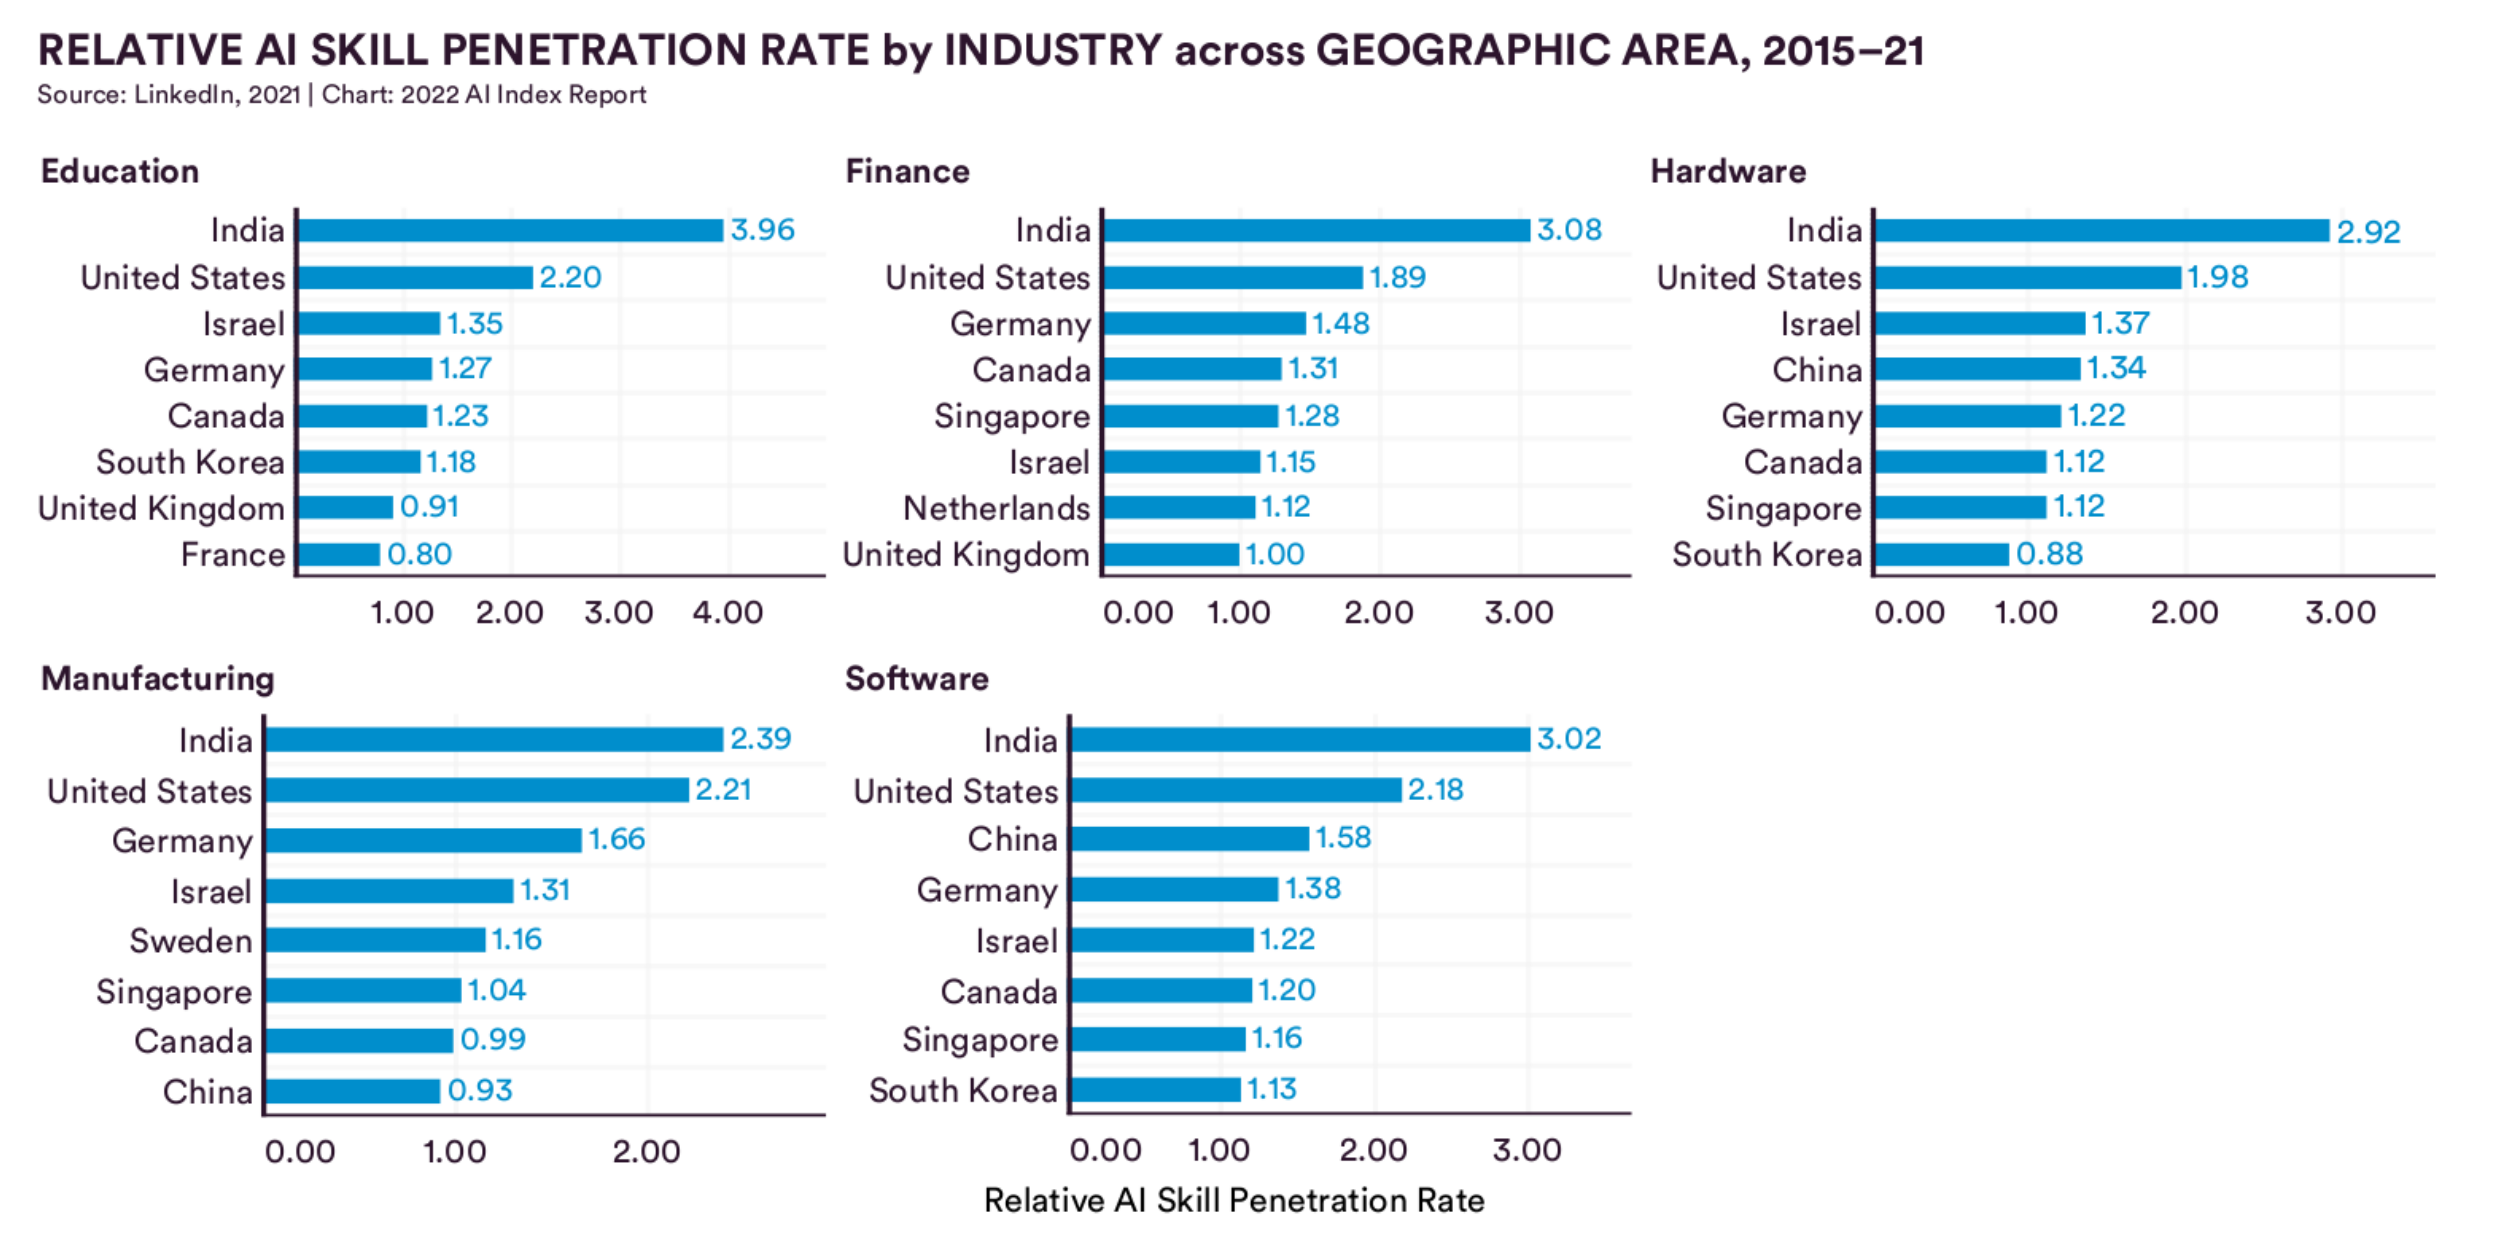
\includegraphics[width=1.0\textwidth]{./progress-of-air-e/outputs/drawing-v00.png}
 %\caption{}
\end{figure}

\end{frame}
}



%%%%%%%%%%%%%%%%%%%%%%%%%%%%%%%%%%%%%%%%%%%%%%%%%%%%%%%%
{
%\paper{Savage N. 2021 in Nature, DOI: doi.org/10.1038/d41586-020-03409-8}
%\paper{Zhang D. et al 2021 in AI 2021 Index Report, Fig 1.1.19 \url{https://aiindex.stanford.edu/report/}}
\paper{AI Index Report 2022, Fig 4.1.10 \url{https://aiindex.stanford.edu/report/}}

\begin{frame}{
%Relative AI skill penetration rate by gender, 2015-2021
Penetraci\'on relativa de habilidades en IA por genero y \'area geogr\'afica, 2015-21
}


\begin{figure}
 \centering
 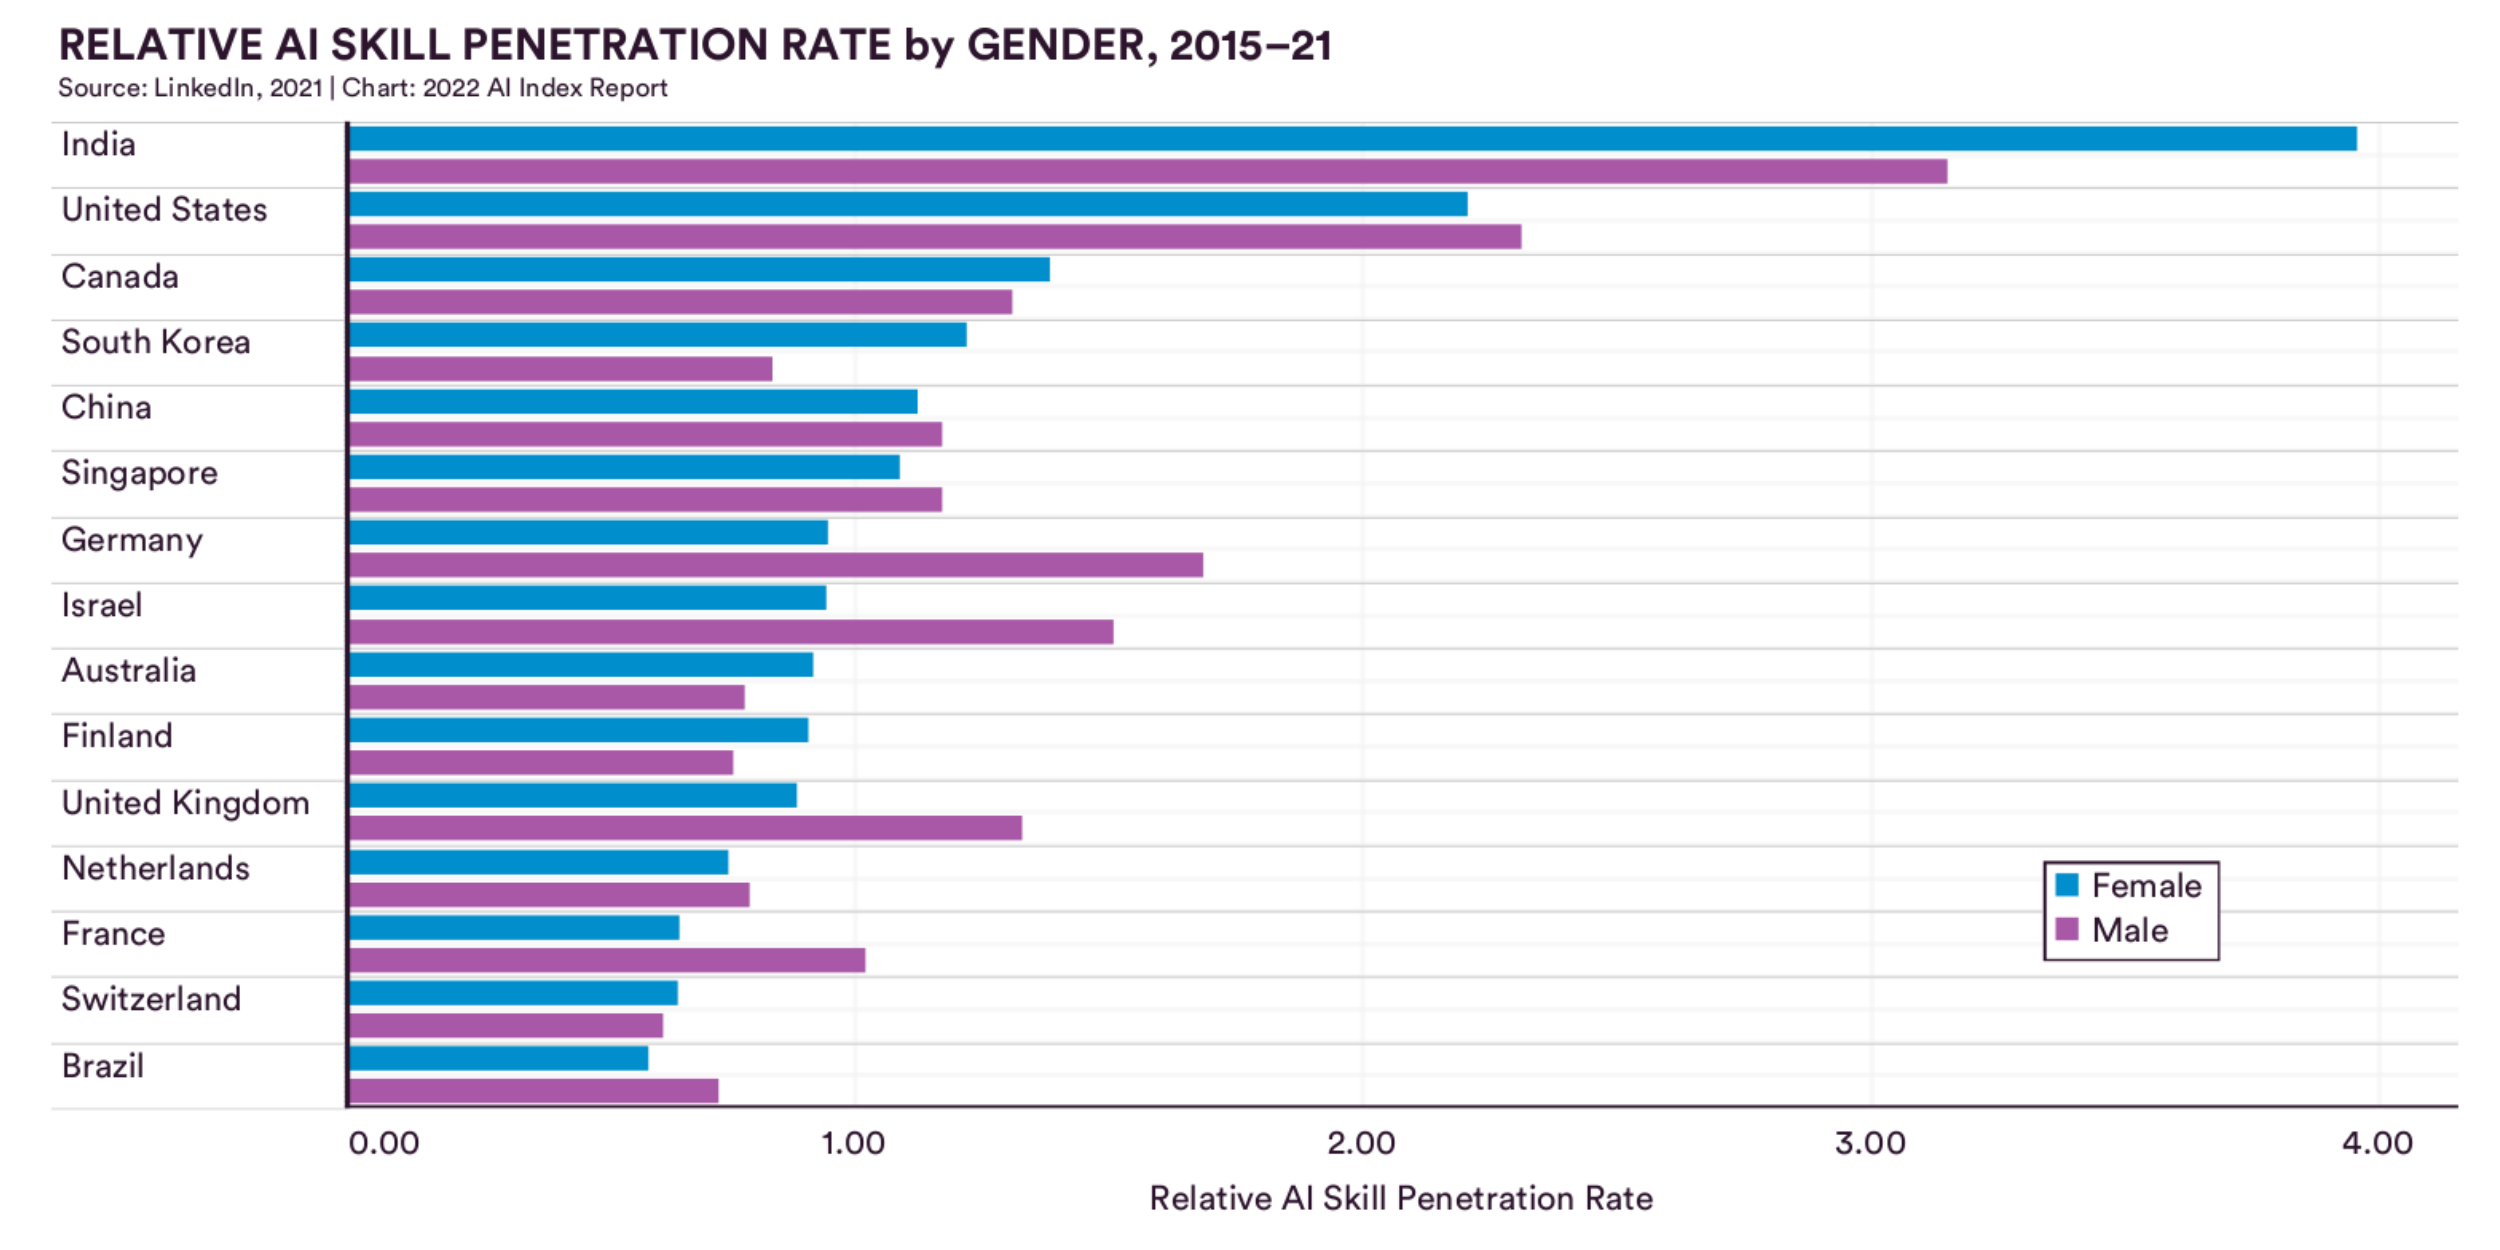
\includegraphics[width=1.0\textwidth]{./progress-of-air-f/outputs/drawing-v00.png}
 %\caption{}
\end{figure}

\end{frame}
}






%%%%%%%%%%%%%%%%%%%%%%%%%%%%%%%%%%%%%%%%%%%%
\section{air4children}


\begin{frame}
      \frametitle{Table of Contents}
      \tableofcontents[currentsection]
\end{frame}


%%%%%%%%%%%%%%%%%%%%%%%%%%%%%%%%%%%%%%%%%%%%%%%%%%%%%%%%
{
%\paper{Lastname N. YEAR in journal of...}
\begin{frame}{What is air4children?}

  \begin{columns}
  \begin{column}{.7\linewidth}

  air4children, Artificial Intelligence and Robotics for Children, aiming  
  \begin{itemize}
    \item to create a more inclusive, affordable and fair participation of children in AI and Robotics,
    \item to create child-centred AI and Robotics curriculums based on Montessori Education, and
    \item to build Open source robots to be affordable and fun. 
  \end{itemize}

    \end{column}


  \begin{column}{.4\linewidth}

      \begin{figure}
        \centering
        \includegraphics[width=0.95\textwidth]{./figures/logo/outputs/drawing-v00.png}
      \end{figure}

    \end{column}
  \end{columns}

\end{frame}
}




%%%%%%%%%%%%%%%%%%%%%%%%%%%%%%%%%%%%%%%%%%%%%
\subsection{Prototyping and piloting Open Source Robots}

%%%%%%%%%%%%%%%%%%%%%%%%%%%%%%%%%%%%%%%%%%%%%%%%%%%%%%%%
{
\paper{Xochicale M. 2014, \it{Proposal of Libre Robotics} }
\begin{frame}{Prototyping Open Source Robots (2013 -- 2017)}
      \begin{figure}
        \centering
        \includegraphics[width=1.0\textwidth]{./figures/air4children-a/outputs/drawing-v00.png}
        %\caption{}
      \end{figure}
\end{frame}
}

%%%%%%%%%%%%%%%%%%%%%%%%%%%%%%%%%%%%%%%%%%%%%%%%%%%%%%%%
{
\paper{Xochicale M. 2015 in Mecate; Parra C. et al. 2016, \it{Otto DIY}}
\begin{frame}{Piloting robot prototypes (2015 -- 2019)}
      \begin{figure}
        \centering
        \includegraphics[width=1.0\textwidth]{./figures/air4children-b/outputs/drawing-v00.png}
        %\caption{}
      \end{figure}
\end{frame}
}

%%%%%%%%%%%%%%%%%%%%%%%%%%%%%%%%%%%%%%%%%%%%%
\subsection{Montessori Education}

%%%%%%%%%%%%%%%%%%%%%%%%%%%%%%%%%%%%%%%%%%%%%%%%%%%%%%%%
{
\paper{Elkin M., Sullivan A, Bers 2014 in Journal of Information and Technology}
\begin{frame}{Montessori Education} 
\vspace{3mm}
%\it{
"The hand is the instrument of the mind."
%} 
%\\
Dr. Maria Montessori (1970-1952).

\vspace{2mm}
    \begin{figure}
        \centering
        \includegraphics[width=1.0\textwidth]{./figures/montessori/outputs/drawing-v00.png}
        %\caption{}
      \end{figure}

Children are participating in creative explorations to develop fine motor skills and to engage in collaborative and teamwork activities. 

\end{frame}
}



%%%%%%%%%%%%%%%%%%%%%%%%%%%%%%%%%%%%%%%%%%%%%%%%%%%%%%%%
{
\paper{Mohammad T. et al., 2017; Harden R. M. 1999 in Journal of Medical Teacher}
\begin{frame}{Spiral Learning Method}

  \begin{figure}
        \centering
        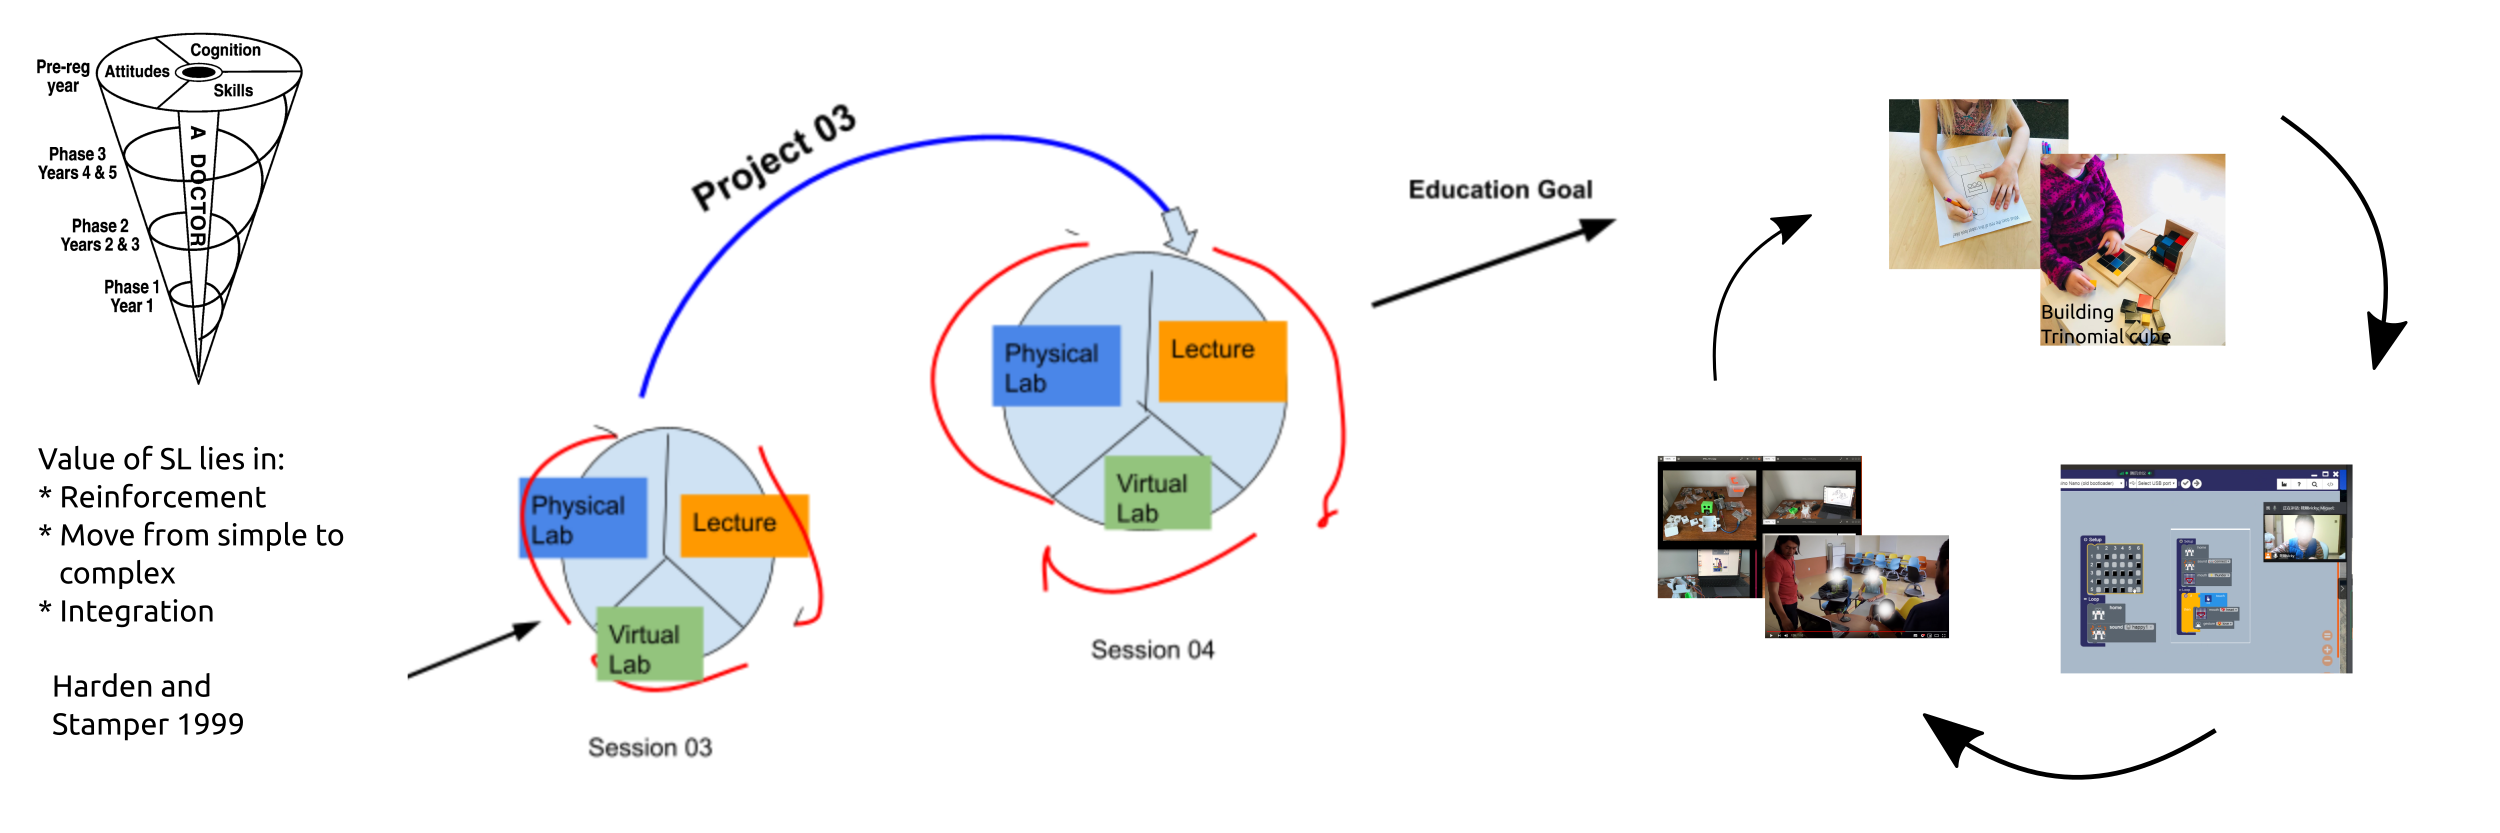
\includegraphics[width=1.0\textwidth]{./figures/teaching-materials/outputs/drawing-v02.png}
        %\caption{}
      \end{figure}
\end{frame}
}

%%%%%%%%%%%%%%%%%%%%%%%%%%%%%%%%%%%%%%%%%%%%
\section{Talleres}

\begin{frame}
      \frametitle{Contenido}
      \tableofcontents[currentsection]
\end{frame}


%%%%%%%%%%%%%%%%%%%%%%%%%%%%%%%%%%%%%%%%%%%%%
\subsection{
Curriculum de cuatro lecciones
}

%%%%%%%%%%%%%%%%%%%%%%%%%%%%%%%%%%%%%%%%%%%%%%%%%%%%%%%%
{
\paper{Badillo-Perez A, Badillo-Perez D, Barco A, Montenegro R, Xochicale M. 2013, Teaching AI and Robotics to Children in a Mexican town, DEI-HRI2023, \url{https://arxiv.org/abs/2303.03956}}

\begin{frame}{Curriculum}
      \begin{figure}
        \centering
        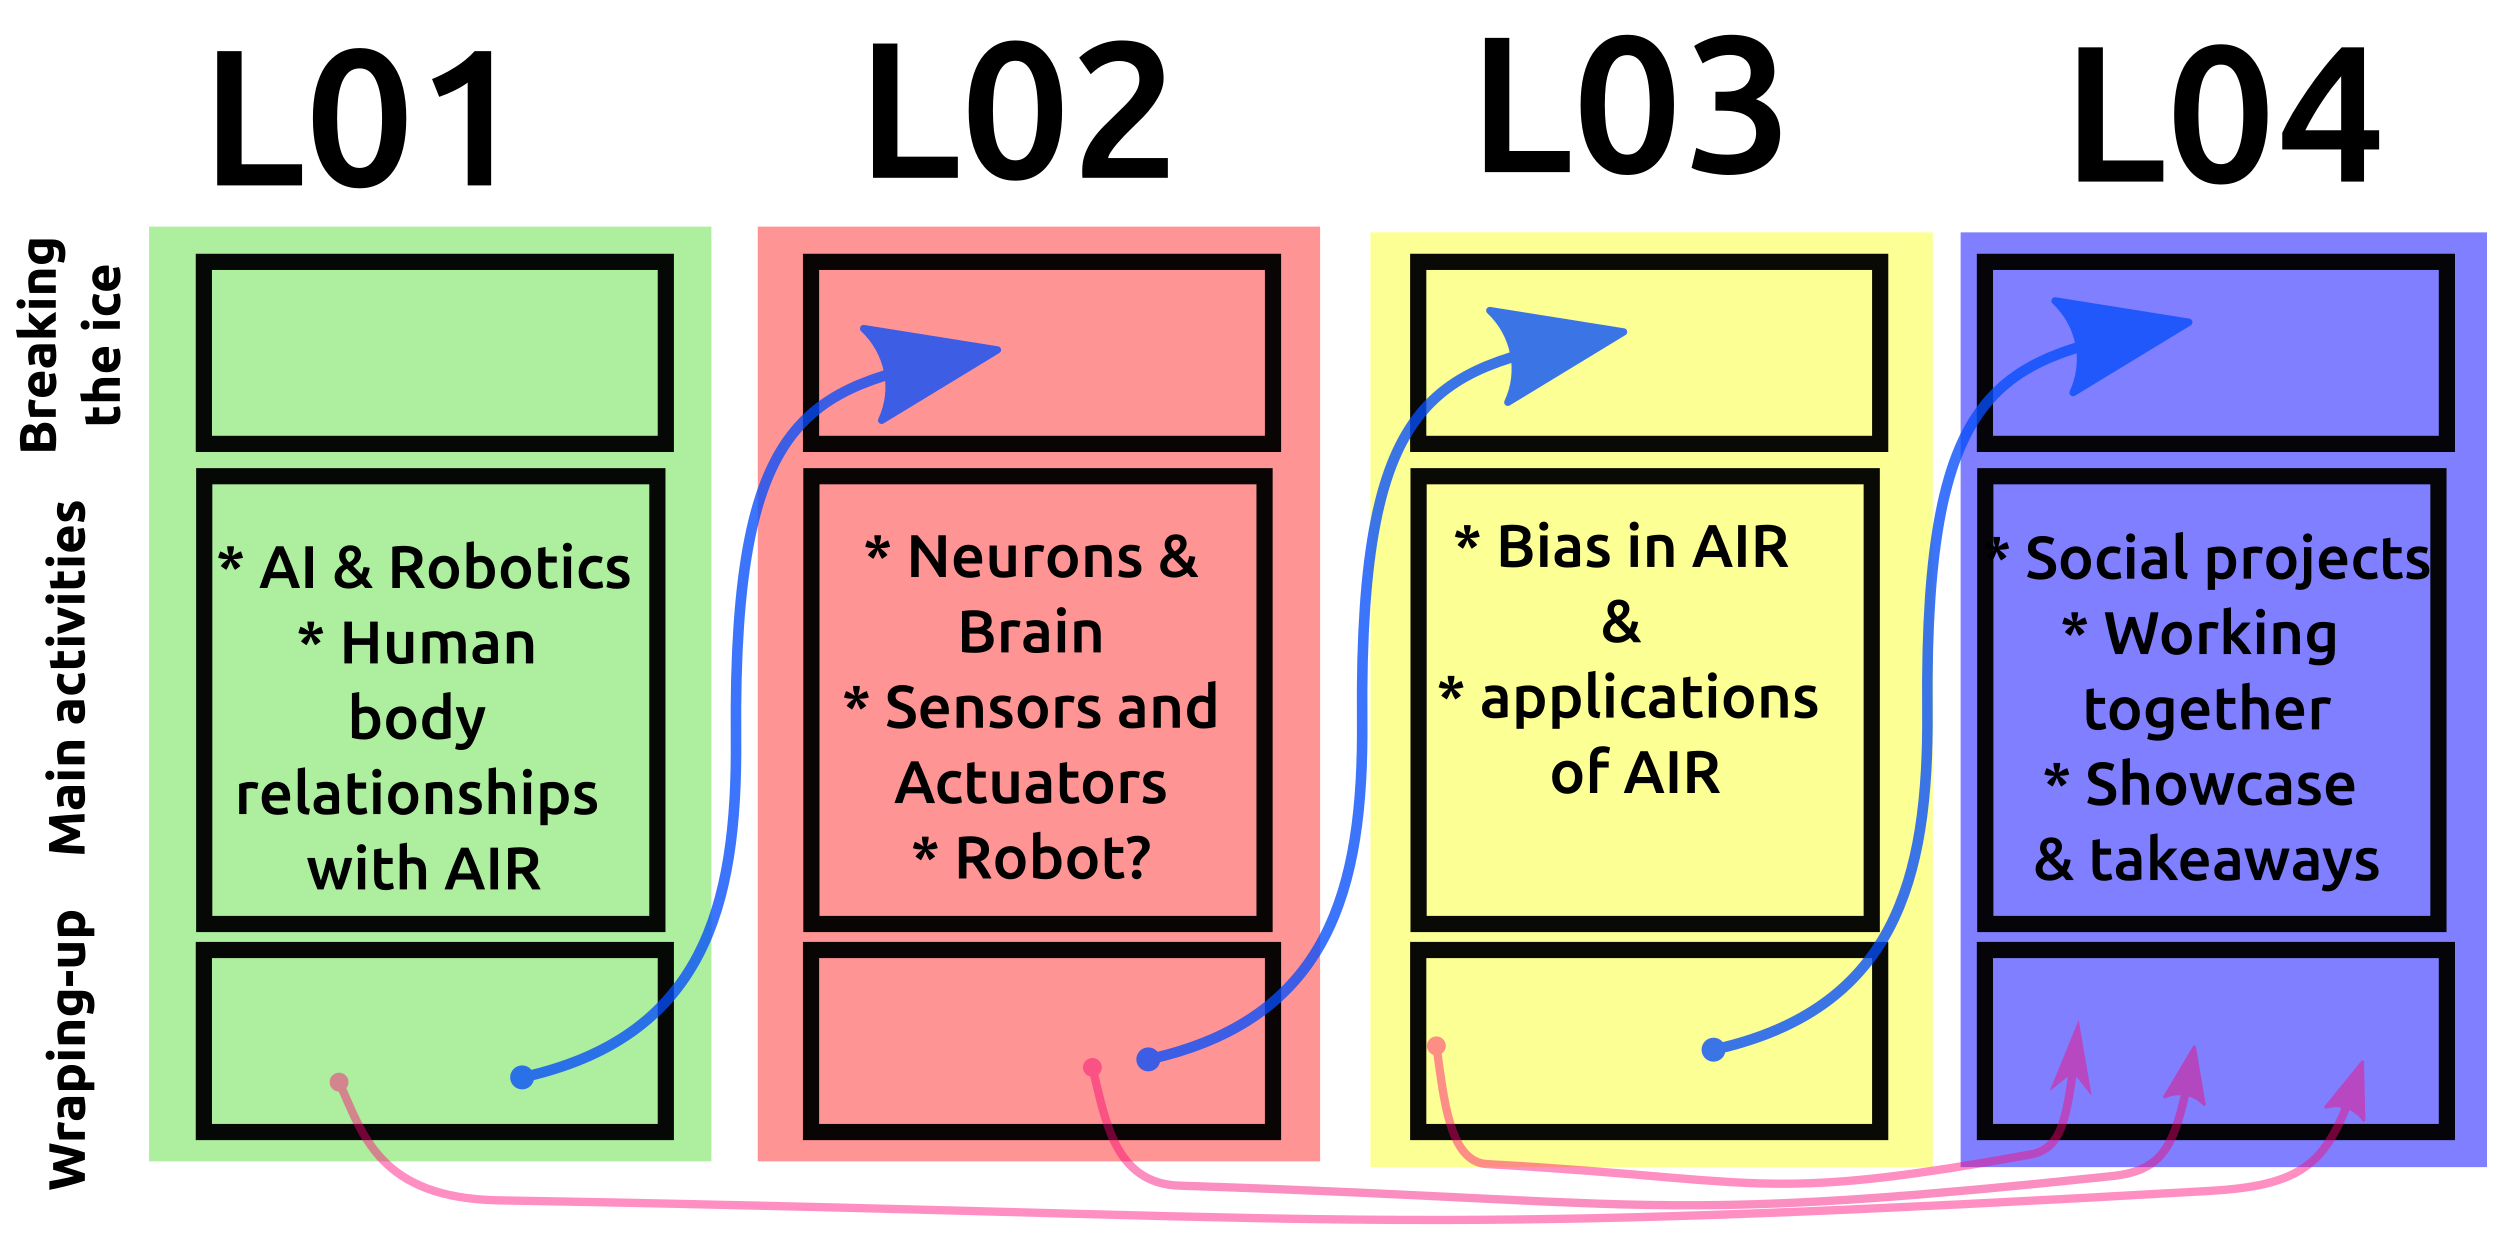
\includegraphics[width=1.0\textwidth]{./curriculum/outputs/drawing-v00.png}
        %\caption{}
      \end{figure}
\end{frame}
}


%%%%%%%%%%%%%%%%%%%%%%%%%%%%%%%%%%%%%%%%%%%%%
\subsection{
Piloteando el curriculum
}

%%%%%%%%%%%%%%%%%%%%%%%%%%%%%%%%%%%%%%%%%%%%%%%%%%%%%%%%
{
\paper{Badillo-Perez A, Badillo-Perez D, Barco A, Montenegro R, \textbf{Xochicale M. 2023}, Teaching AI and Robotics to Children in a Mexican town, DEI-HRI2023, \url{https://arxiv.org/abs/2303.03956}}

\begin{frame}{Participantes}

\begin{itemize}
\item 14 participantes de los cuales 10 atendieron el taller, 6 hombres y 4 mujeres (de edad en a\~nos: promedio=8 and desviaci\'on estandar=$\pm$1.61)     
\item 4 instructores con diferentes niveles de experiencia en ense\~nanza a ni\~nos y jovenes.
\end{itemize}

\end{frame}
}




%%%%%%%%%%%%%%%%%%%%%%%%%%%%%%%%%%%%%%%%%%%%%%%%%%%%%%%%
{
\paper{Badillo-Perez A, Badillo-Perez D, Barco A, Montenegro R, \textbf{Xochicale M. 2023}, Teaching AI and Robotics to Children in a Mexican town, DEI-HRI2023, \url{https://arxiv.org/abs/2303.03956}}

\begin{frame}{
%Piloting workshop: Coding and bingo activities
Piloteando talleres: Codificando y el juego de bingo
}
      \begin{figure}
        \centering
        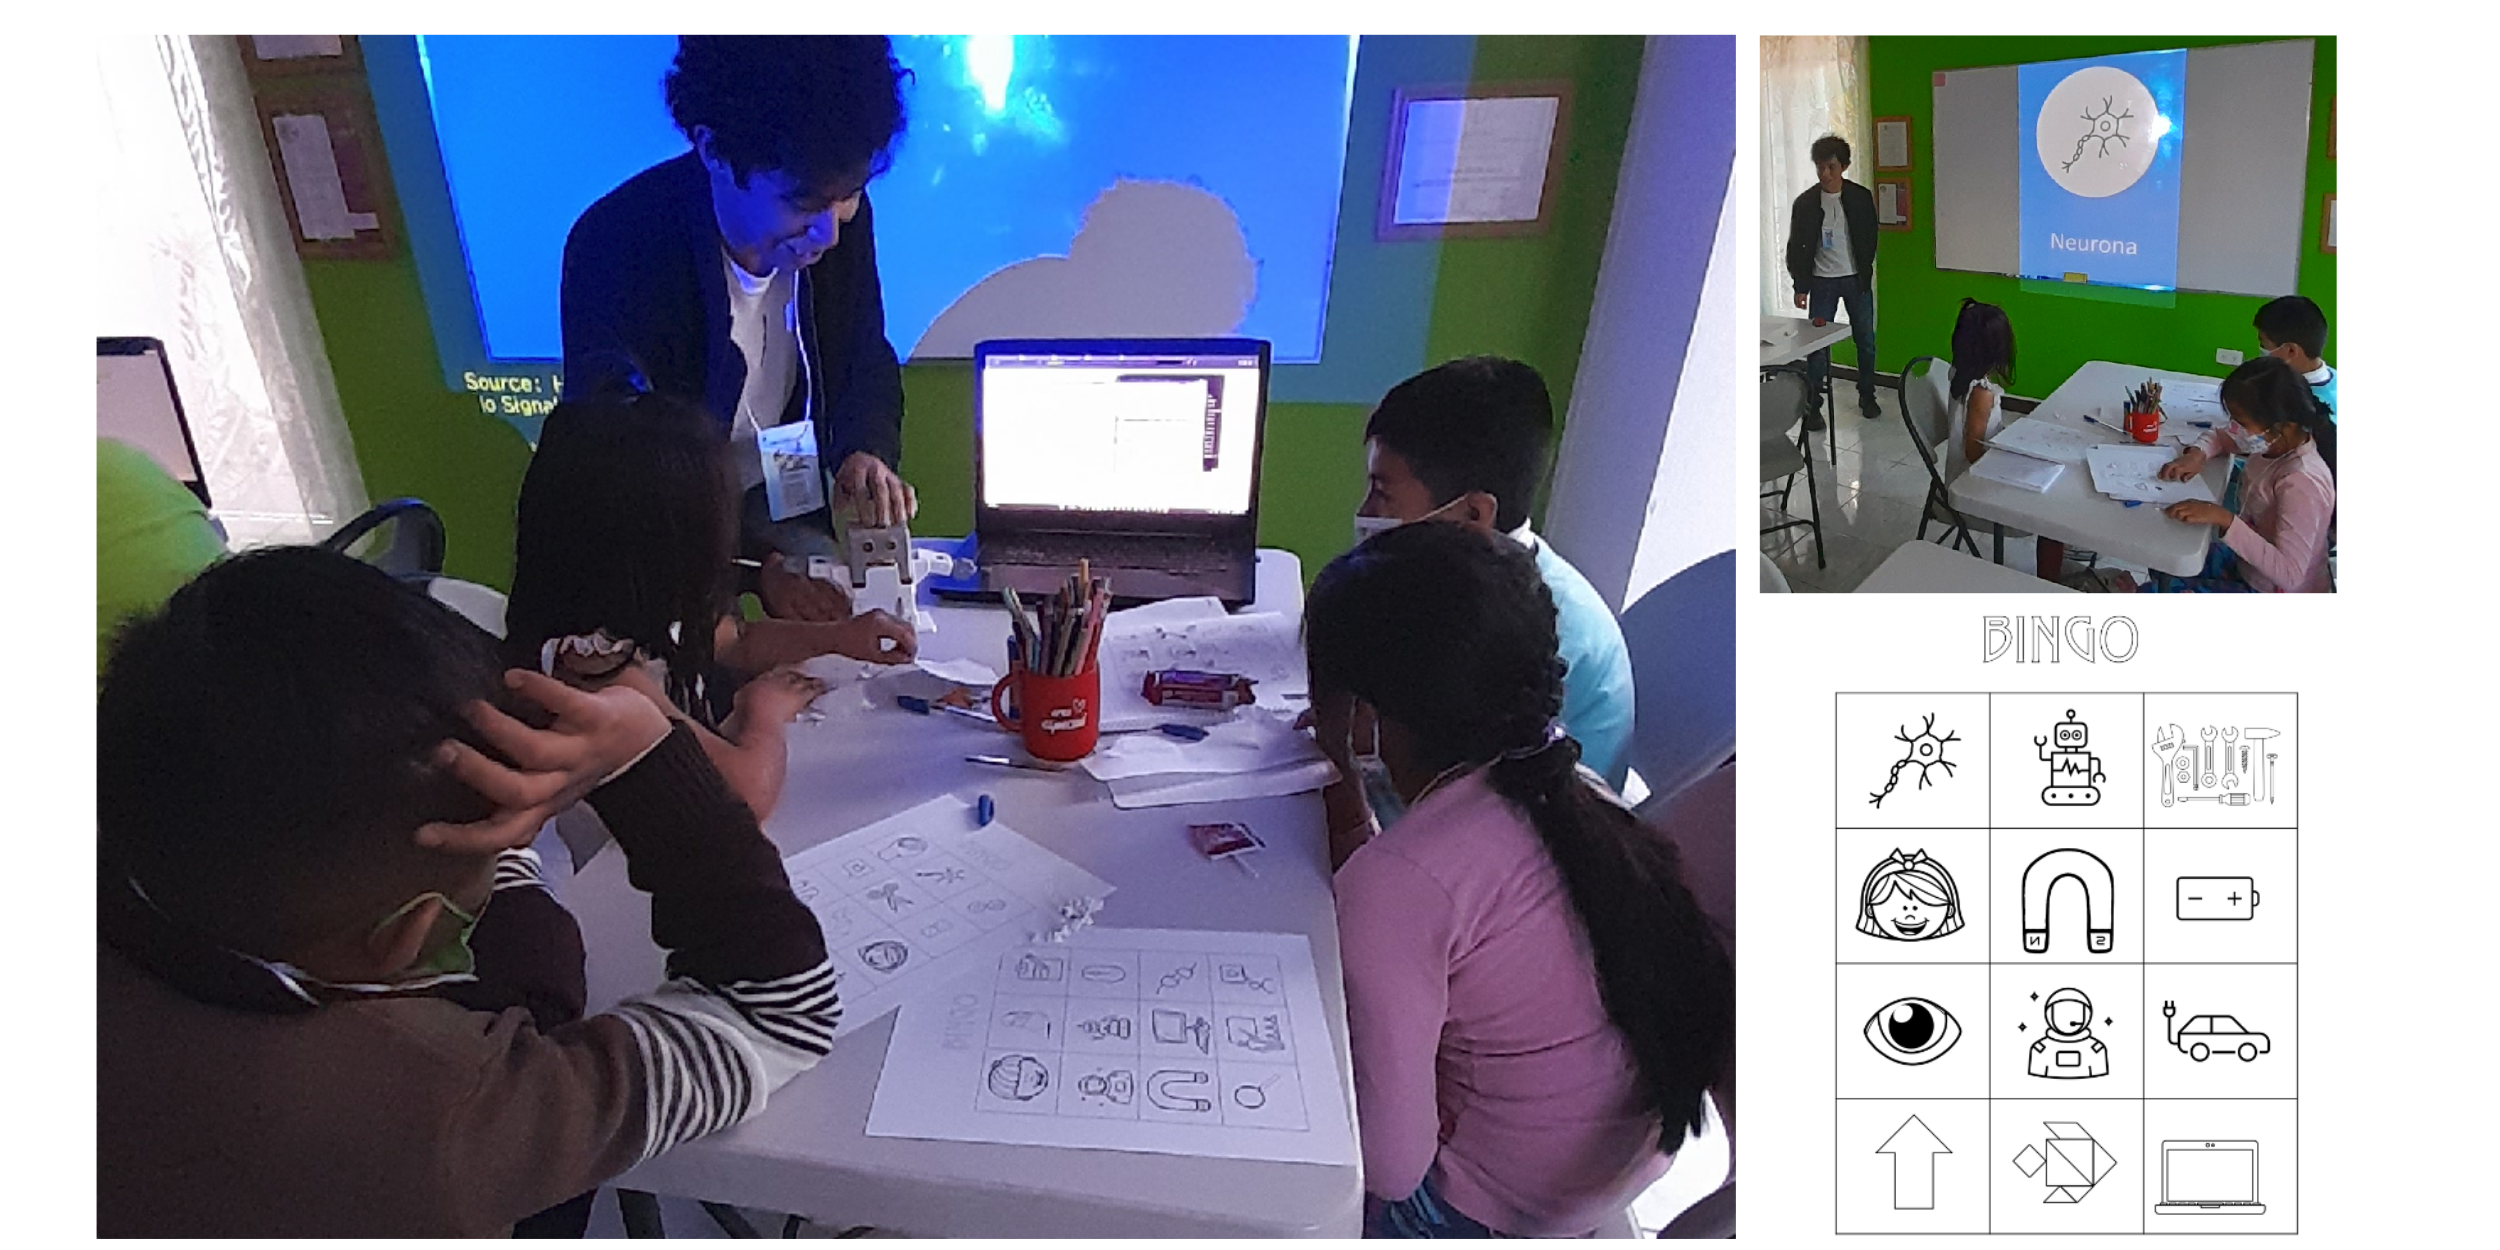
\includegraphics[width=1.0\textwidth]{./pilot-workshop-a/outputs/drawing-v00.png}
        %\caption{}
      \end{figure}
\end{frame}
}



%%%%%%%%%%%%%%%%%%%%%%%%%%%%%%%%%%%%%%%%%%%%%%%%%%%%%%%%
{

\paper{Badillo-Perez A, Badillo-Perez D, Barco A, Montenegro R, \textbf{Xochicale M. 2023}, Teaching AI and Robotics to Children in a Mexican town, DEI-HRI2023, \url{https://arxiv.org/abs/2303.03956}}

\begin{frame}{
%Piloting workshop: Teaching activities
Piloteando talleres: Actividades de ense\~nanza
}
      \begin{figure}
        \centering
        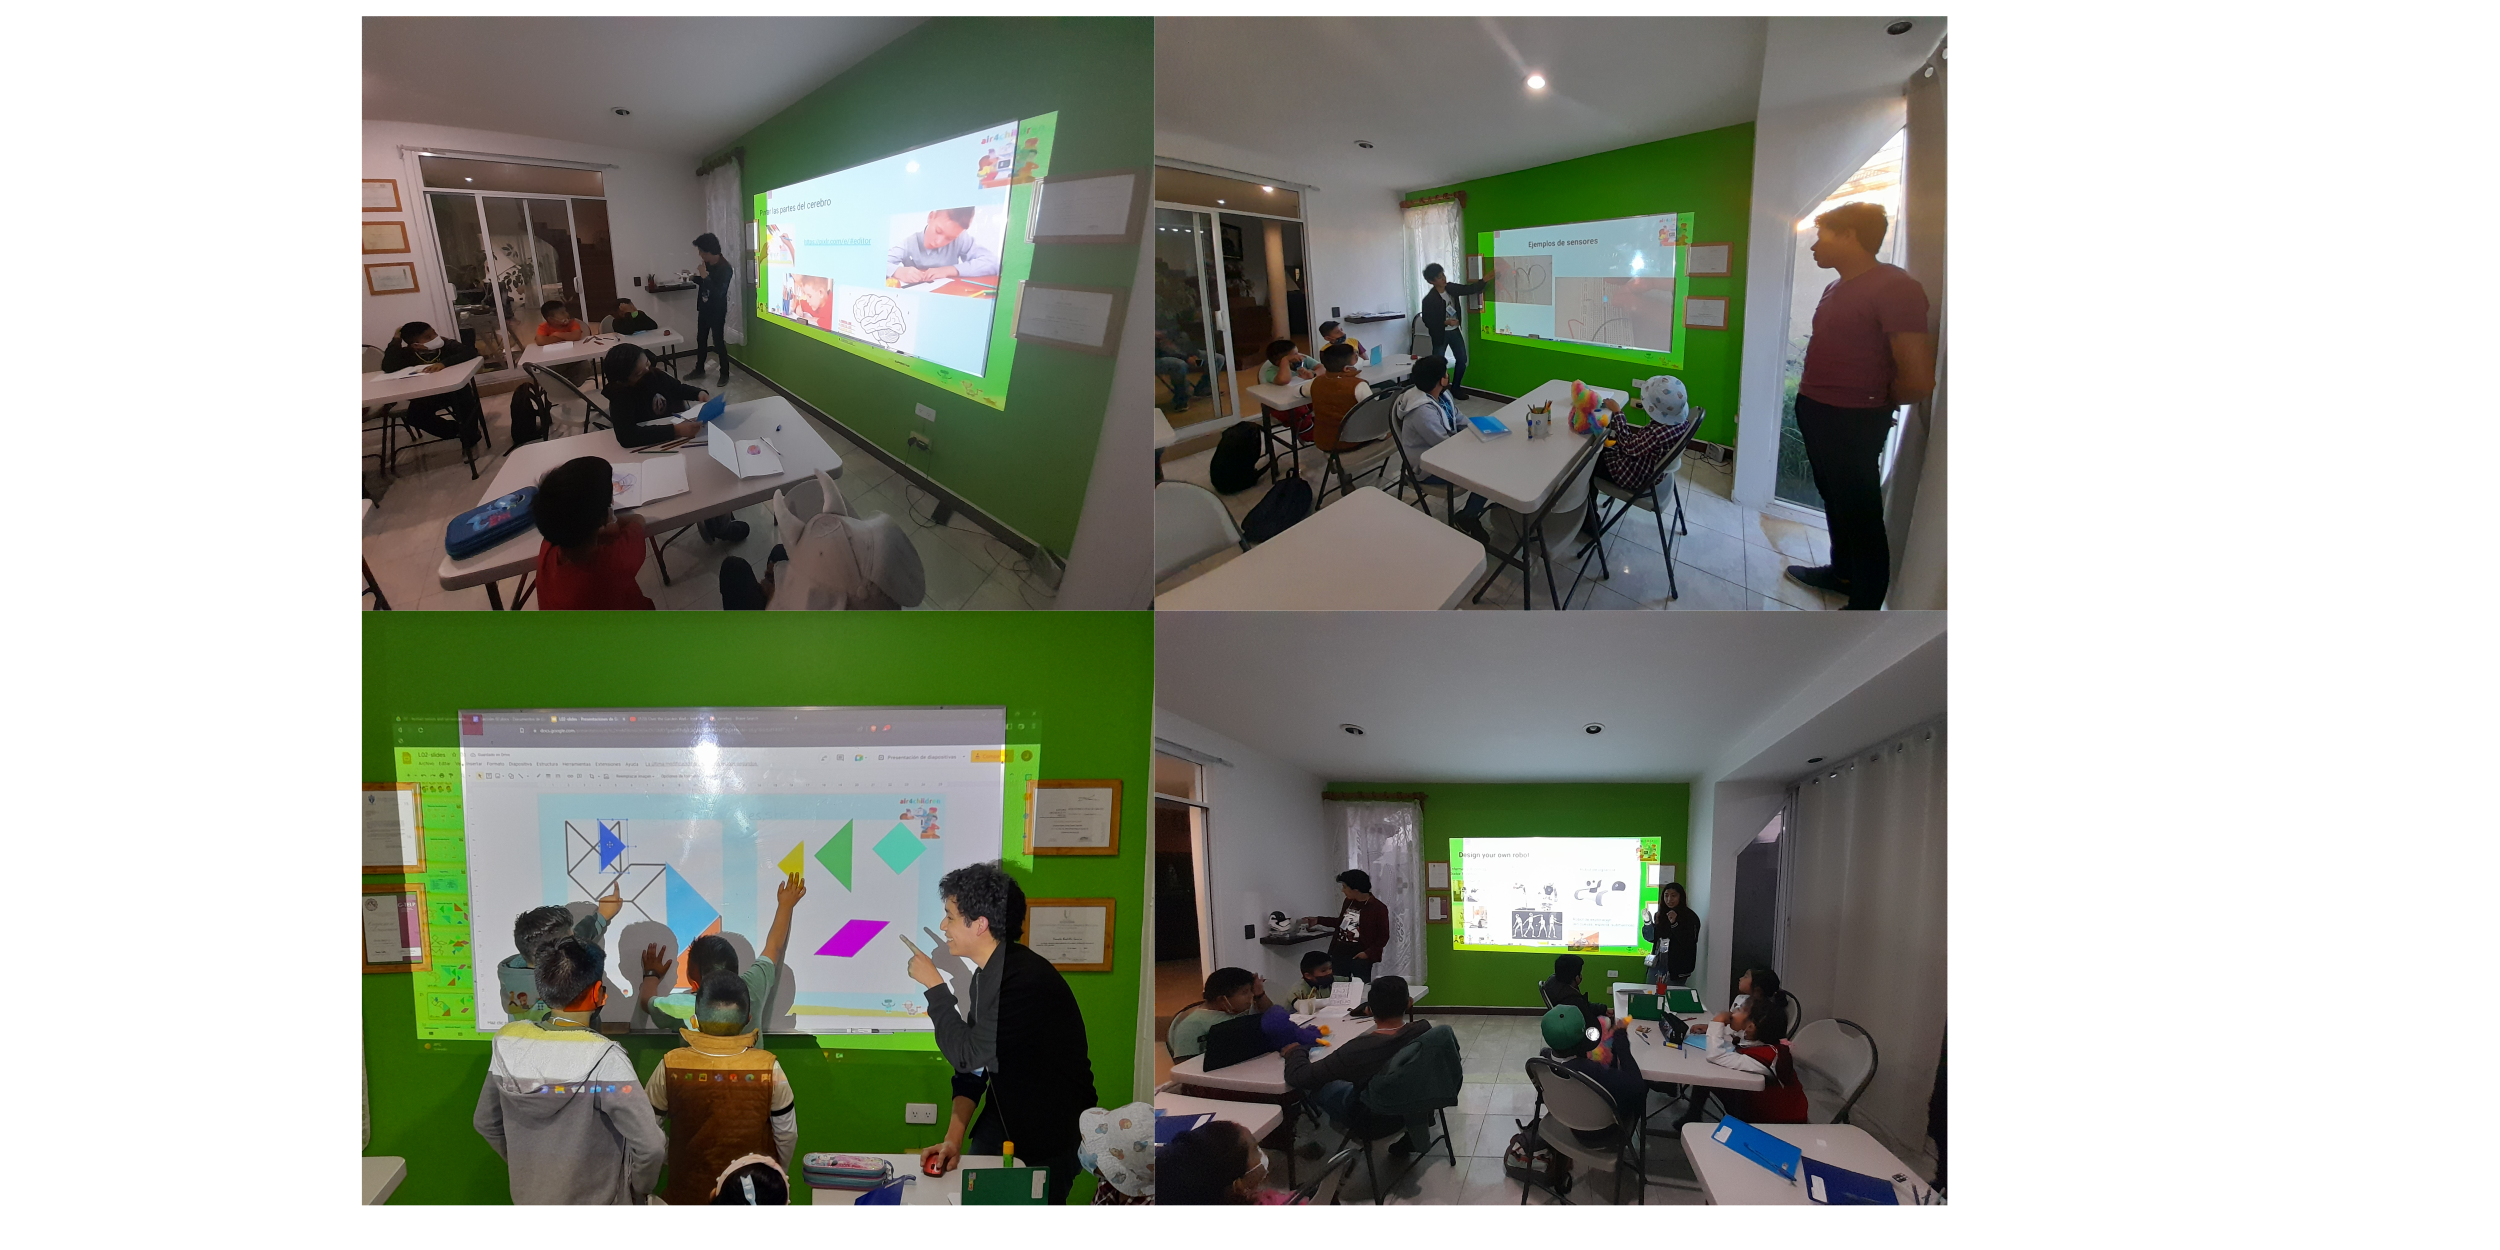
\includegraphics[width=1.0\textwidth]{./pilot-workshop-b/outputs/drawing-v00.png}
        %\caption{}
      \end{figure}
\end{frame}
}

%%%%%%%%%%%%%%%%%%%%%%%%%%%%%%%%%%%%%%%%%%%%%%%%%%%%%%%%
{

\paper{Badillo-Perez A, Badillo-Perez D, Barco A, Montenegro R, \textbf{Xochicale M. 2023}, Teaching AI and Robotics to Children in a Mexican town, DEI-HRI2023, \url{https://arxiv.org/abs/2303.03956}}

\begin{frame}{
%Piloting workshop: Group activities
Piloteando talleres: Actividades en grupo
}
      \begin{figure}
        \centering
        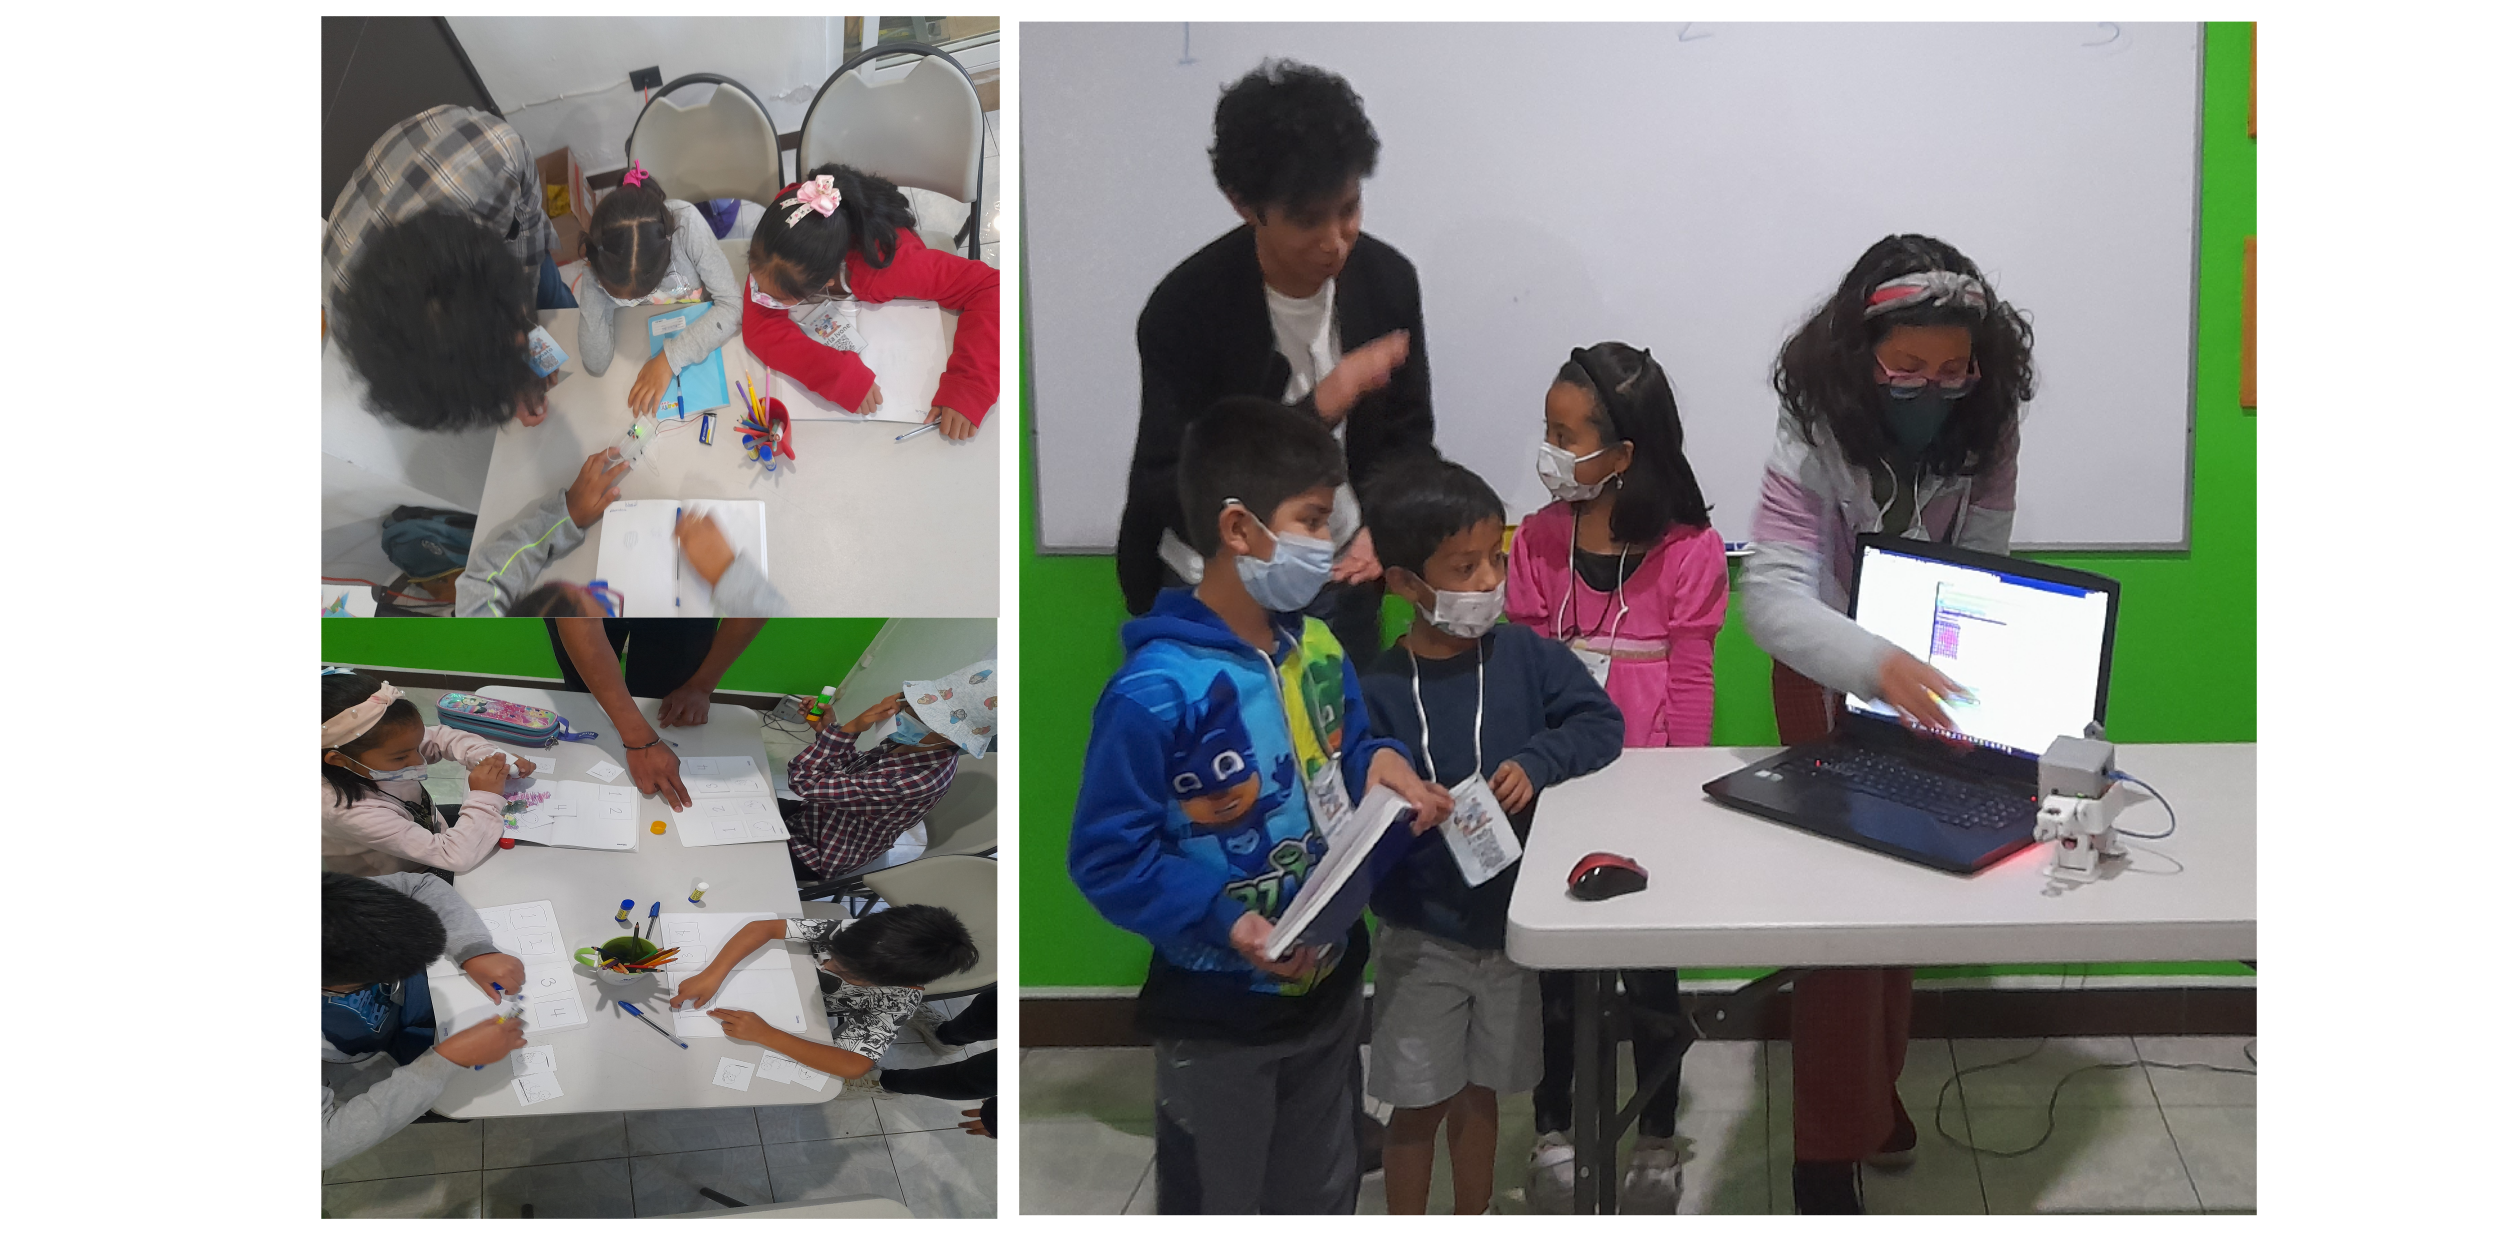
\includegraphics[width=1.0\textwidth]{./pilot-workshop-c/outputs/drawing-v00.png}
        %\caption{}
      \end{figure}
\end{frame}
}

%%%%%%%%%%%%%%%%%%%%%%%%%%%%%%%%%%%%%%%%%%%%%
\subsection{
%Results of the survey
Resultados de las encuestas
}

%%%%%%%%%%%%%%%%%%%%%%%%%%%%%%%%%%%%%%%%%%%%%%%%%%%%%%%%
{

\paper{Badillo-Perez A, Badillo-Perez D, Barco A, Montenegro R, \textbf{Xochicale M. 2023}, Teaching AI and Robotics to Children in a Mexican town, DEI-HRI2023, \url{https://arxiv.org/abs/2303.03956}}

\begin{frame}{
%Survey results
Resultados de las encuestas
}
      \begin{figure}
        \centering
        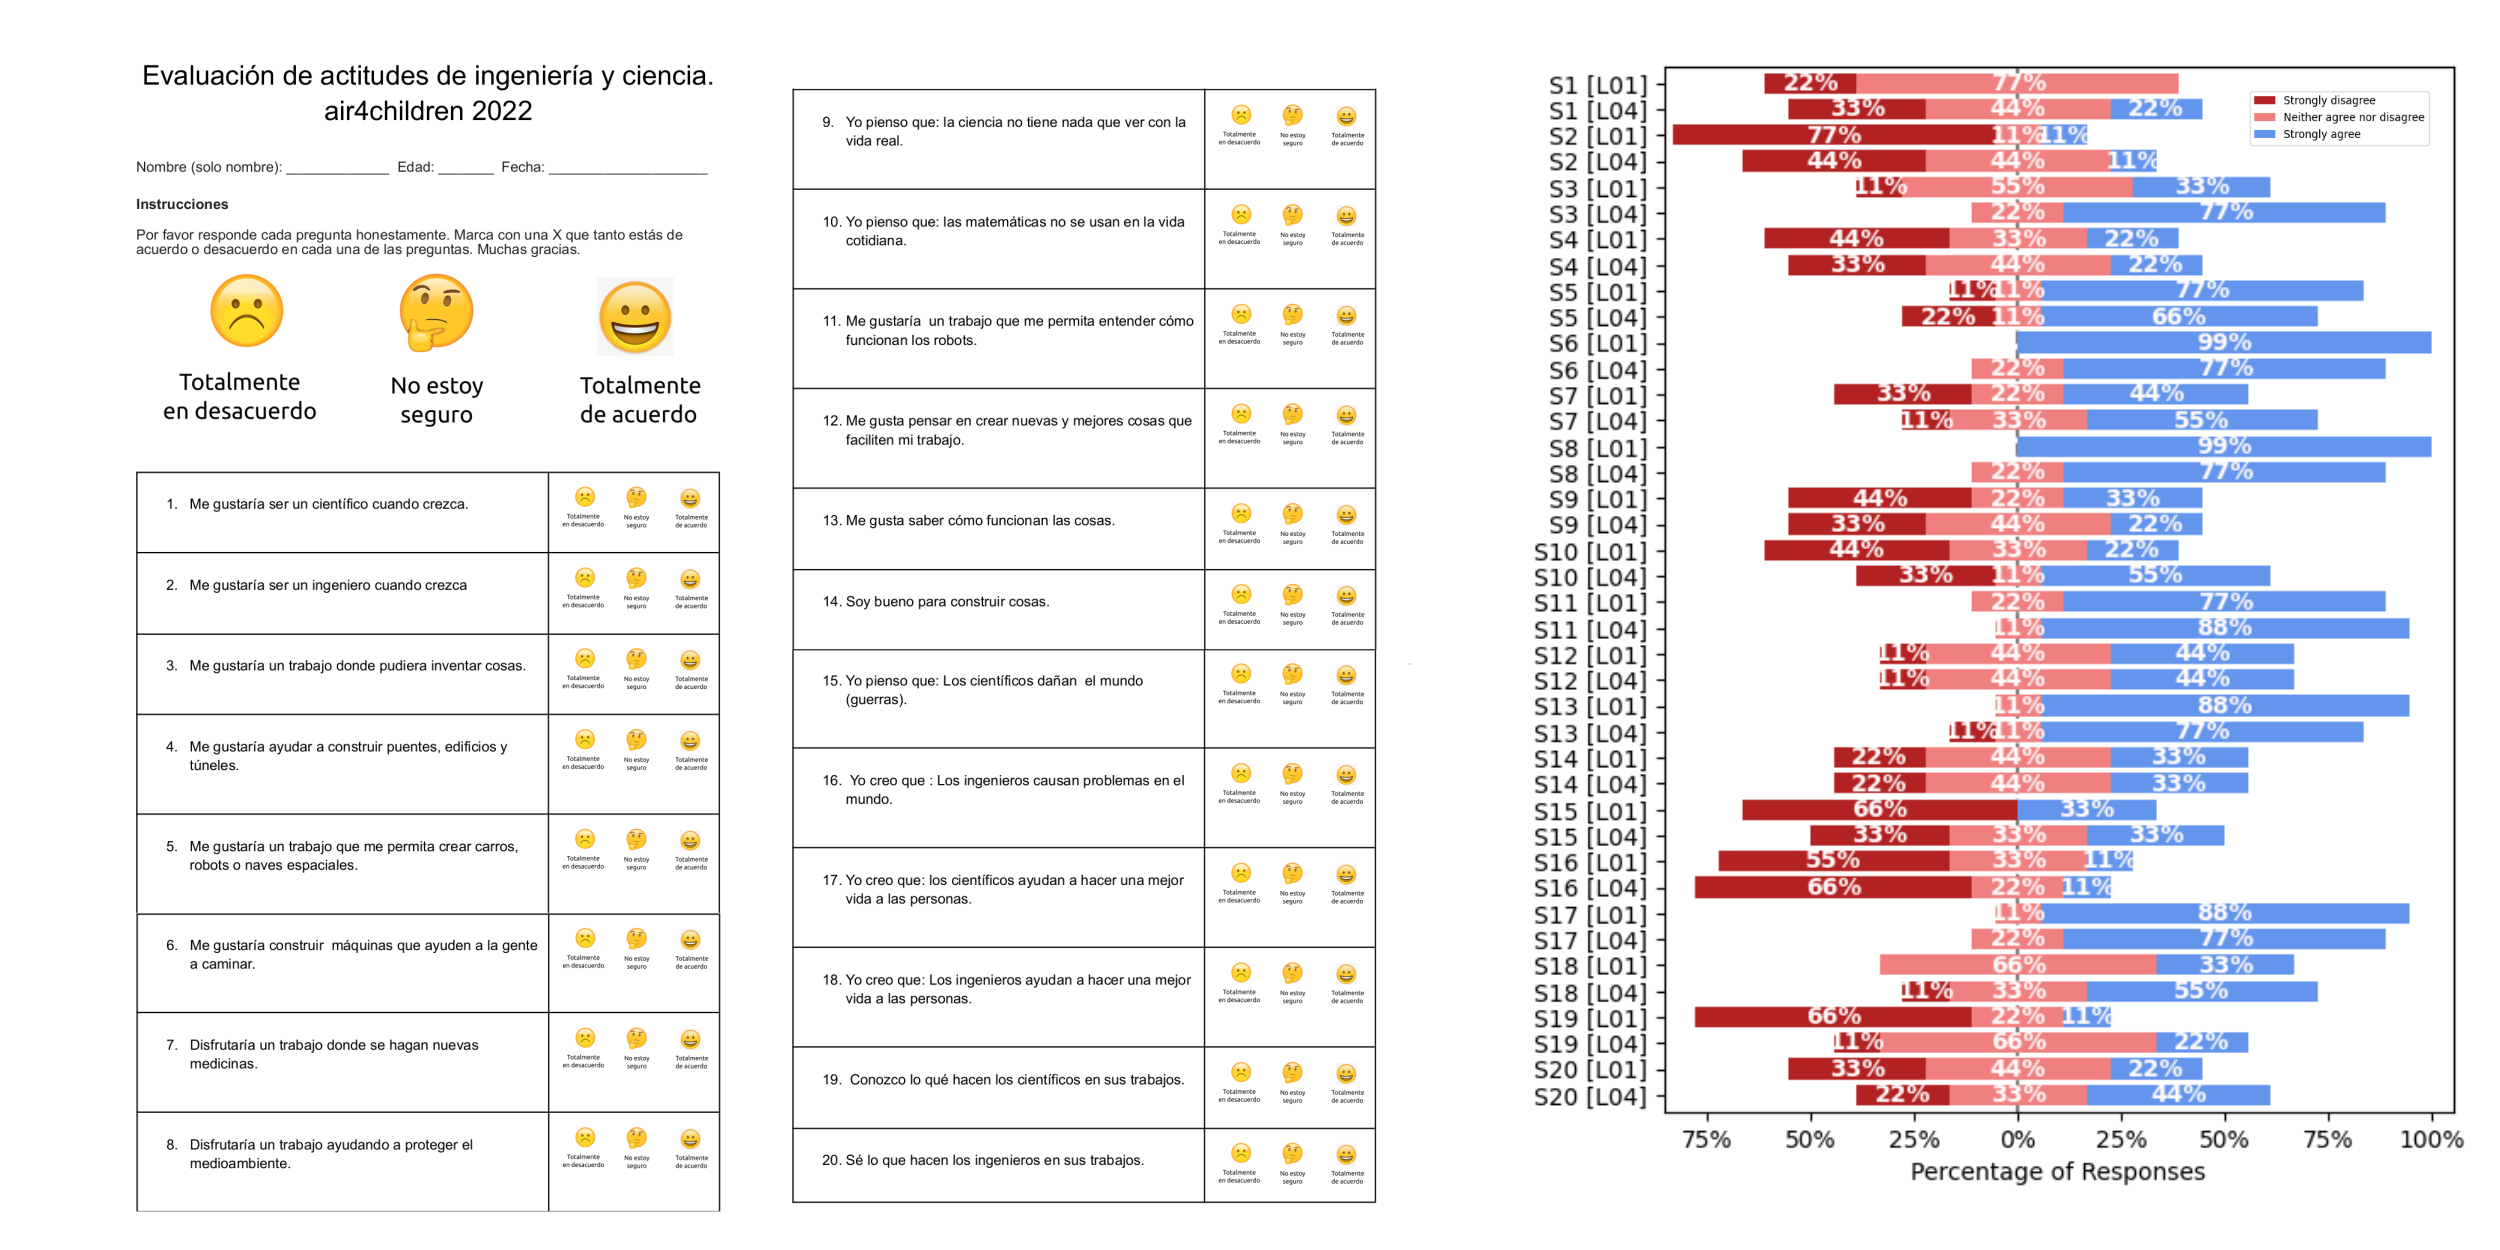
\includegraphics[width=1.0\textwidth]{./survey-results/outputs/drawing-v00.png}
        %\caption{}
      \end{figure}
\end{frame}
}



%%%%%%%%%%%%%%%%%%%%%%%%%%%%%%%%%%%%%%%%%%%%%%%%%%%%%%%%
{
\paper{Badillo-Perez A, Badillo-Perez D, Barco A, Montenegro R, \textbf{Xochicale M. 2023}, Teaching AI and Robotics to Children in a Mexican town, DEI-HRI2023, \url{https://arxiv.org/abs/2303.03956}}

\begin{frame}{An\'alisis estad\'istico}

\begin{itemize}
%\item A Wilcoxon T test was used to analyze the results of the survey before and after the survey to see if the engineering attitudes had a significant effect on pre and post survey of the workshop.
\item Prueba Wilcoxon T se uso para analizar los resultados de las encuentas antes y despu\'es para probar si las actitudes de ingenierian tuvieron un efecto significativo.
%\item The average survey before the test was lower ($\mu$ = 2.194500 $\pm \sigma$ 0.558367 ) compared to the posttest results ($\mu$ = 2.239500 $\pm \sigma$= 0.396796).
\item El promedio de la prueba antes de la encuesta es menor ($\mu$ = 2.194500 $\pm \sigma$ 0.558367 ) comparado a la prueba despu\'es de la encuesta ($\mu$ = 2.239500 $\pm \sigma$= 0.396796).
%\item There was no statistically significant in the increase of attitudes towards engineering (t=53.5, p= 0.45).
\item Los resultados no muestra un resultado estadisticamente significativo en el incremento de la atidudes hacia ingenier\'ia y ciencia (t=53.5, p= 0.45).
\end{itemize}

%See Appendix section for reproducible Jupyter notebooks of statistical analysis and plots.
Ver el apendice con codigo en Jupyter para su replicaci\'on.

\end{frame}
}


%%%%%%%%%%%%%%%%%%%%%%%%%%%%%%%%%%%%%%%%%%%%
\section{Conclusiones y trabajo futuro}

\begin{frame}
      \frametitle{Contenido}
      \tableofcontents[currentsection]
\end{frame}

%%%%%%%%%%%%%%%%%%%%%%%%%%%%%%%%%%%%%%%%%%%%%%%%%%%%%%%%
{
%\paper{Lastname N. YEAR in journal of...}
\begin{frame}{Conclusiones y trabajo futuro}

  \begin{columns}
  \begin{column}{.75\linewidth}

  \textbf{Conclusiones}   

  \begin{itemize}
    %\item Applied Montessory Education and spiral education to design child-based curriculumns in AI and Robotics
    \item Se aplico el m\'etodo Montessory y m\'etodo espiral para dise\~nar curriculms de IA y Rob\'otica para ni\~nos
    %\item Piloted a workshop with 14 participants of 4 lessons surveying attitudes with liker chart
    \item Se piloteo un taller con un curriculum de 4 lecciones, con 14 participantes, evaluando resultados de actitudes de ingenier\'ia y ciencia usando Wilcoxon and escala liker 
  \end{itemize}

  \textbf{Trabajo futuro}
  \begin{itemize}
    \item Mejorar las encuetas y el anal\'isis estad\'istico 
    \item Pilotear el taller con un major n\'umero de participantes
    \item Aplicar a esquemas de financiamiento
    \item Iniciar relaciones legisladores internaciones que promuevan el proyecto air4children
\end{itemize}

    \end{column}


  \begin{column}{.3\linewidth}

      \begin{figure}
        \centering
        
\includegraphics[width=0.9\textwidth]{./logo/outputs/drawing-v00.png}
      \end{figure}

    \end{column}
  \end{columns}

\end{frame}
}


%%%%%%%%%%%%%%%%%%%%%%%%%%%%%%%%%%%%%%%%%%%%%%%%%%%%%%%%%
%{
%%\paper{Lastname N. YEAR in journal of...}
%\begin{frame}{Acknowledgements}
%
%  \begin{figure}
%  \centering
%  \includegraphics[width=1.0\textwidth]{./figures/team/outputs/drawing-v00.png}
%  \end{figure}
%
%\end{frame}
%}
%



%\begin{frame}
%  Thanks \\
%  Questions?
%\end{frame}

\maketitle

\end{document}
